\documentclass[a4paper]{article}
\usepackage{geometry}
\geometry{a4paper,top=3cm,bottom=3cm,left=3cm,right=3cm}
\usepackage{graphicx}
\usepackage{wrapfig}
\usepackage{longtable}
\usepackage{hyperref}
\hypersetup{
	unicode=true,
	pdfborder={0 0 0},
	breaklinks=true
}
\usepackage{dialogue}
\usepackage{polyglossia}
\usepackage{color, colortbl}
\usepackage[dvipsnames]{xcolor}
\definecolor{dark-gray}{gray}{0.30}
\definecolor{light-gray}{gray}{0.60}
\definecolor{light-light-gray}{gray}{0.90}

\usepackage{float}
\usepackage[labelformat=empty]{caption}


\renewcommand*\contentsname{Summary}

\begin{document}

\thispagestyle{empty}
{

	\begin{figure}
		\begin{minipage}{0.5\textwidth}
			\centering
			
\includegraphics[width=0.6\linewidth]{images/frontespizio/unimi_logo.png}
		\end{minipage}\hfill
		\begin{minipage}{0.5\textwidth}
			\centering
			
\includegraphics[width=0.6\linewidth]{images/frontespizio/pong_logo.png}
		\end{minipage}
	\end{figure}

	\vspace*{0.6cm}
	\begin{center}
		\Huge LEVEL DESIGN DOCUMENT\\
	\end{center}
	
	\vspace{2mm}
	\begin{center}
		\Huge \textbf{STRANGER THINGS}\\
		\Huge {Secrets of the Upside Down}\\
		\huge \textbf{Level 15 - The Giant Chasm}\\
		\vspace*{10mm}
		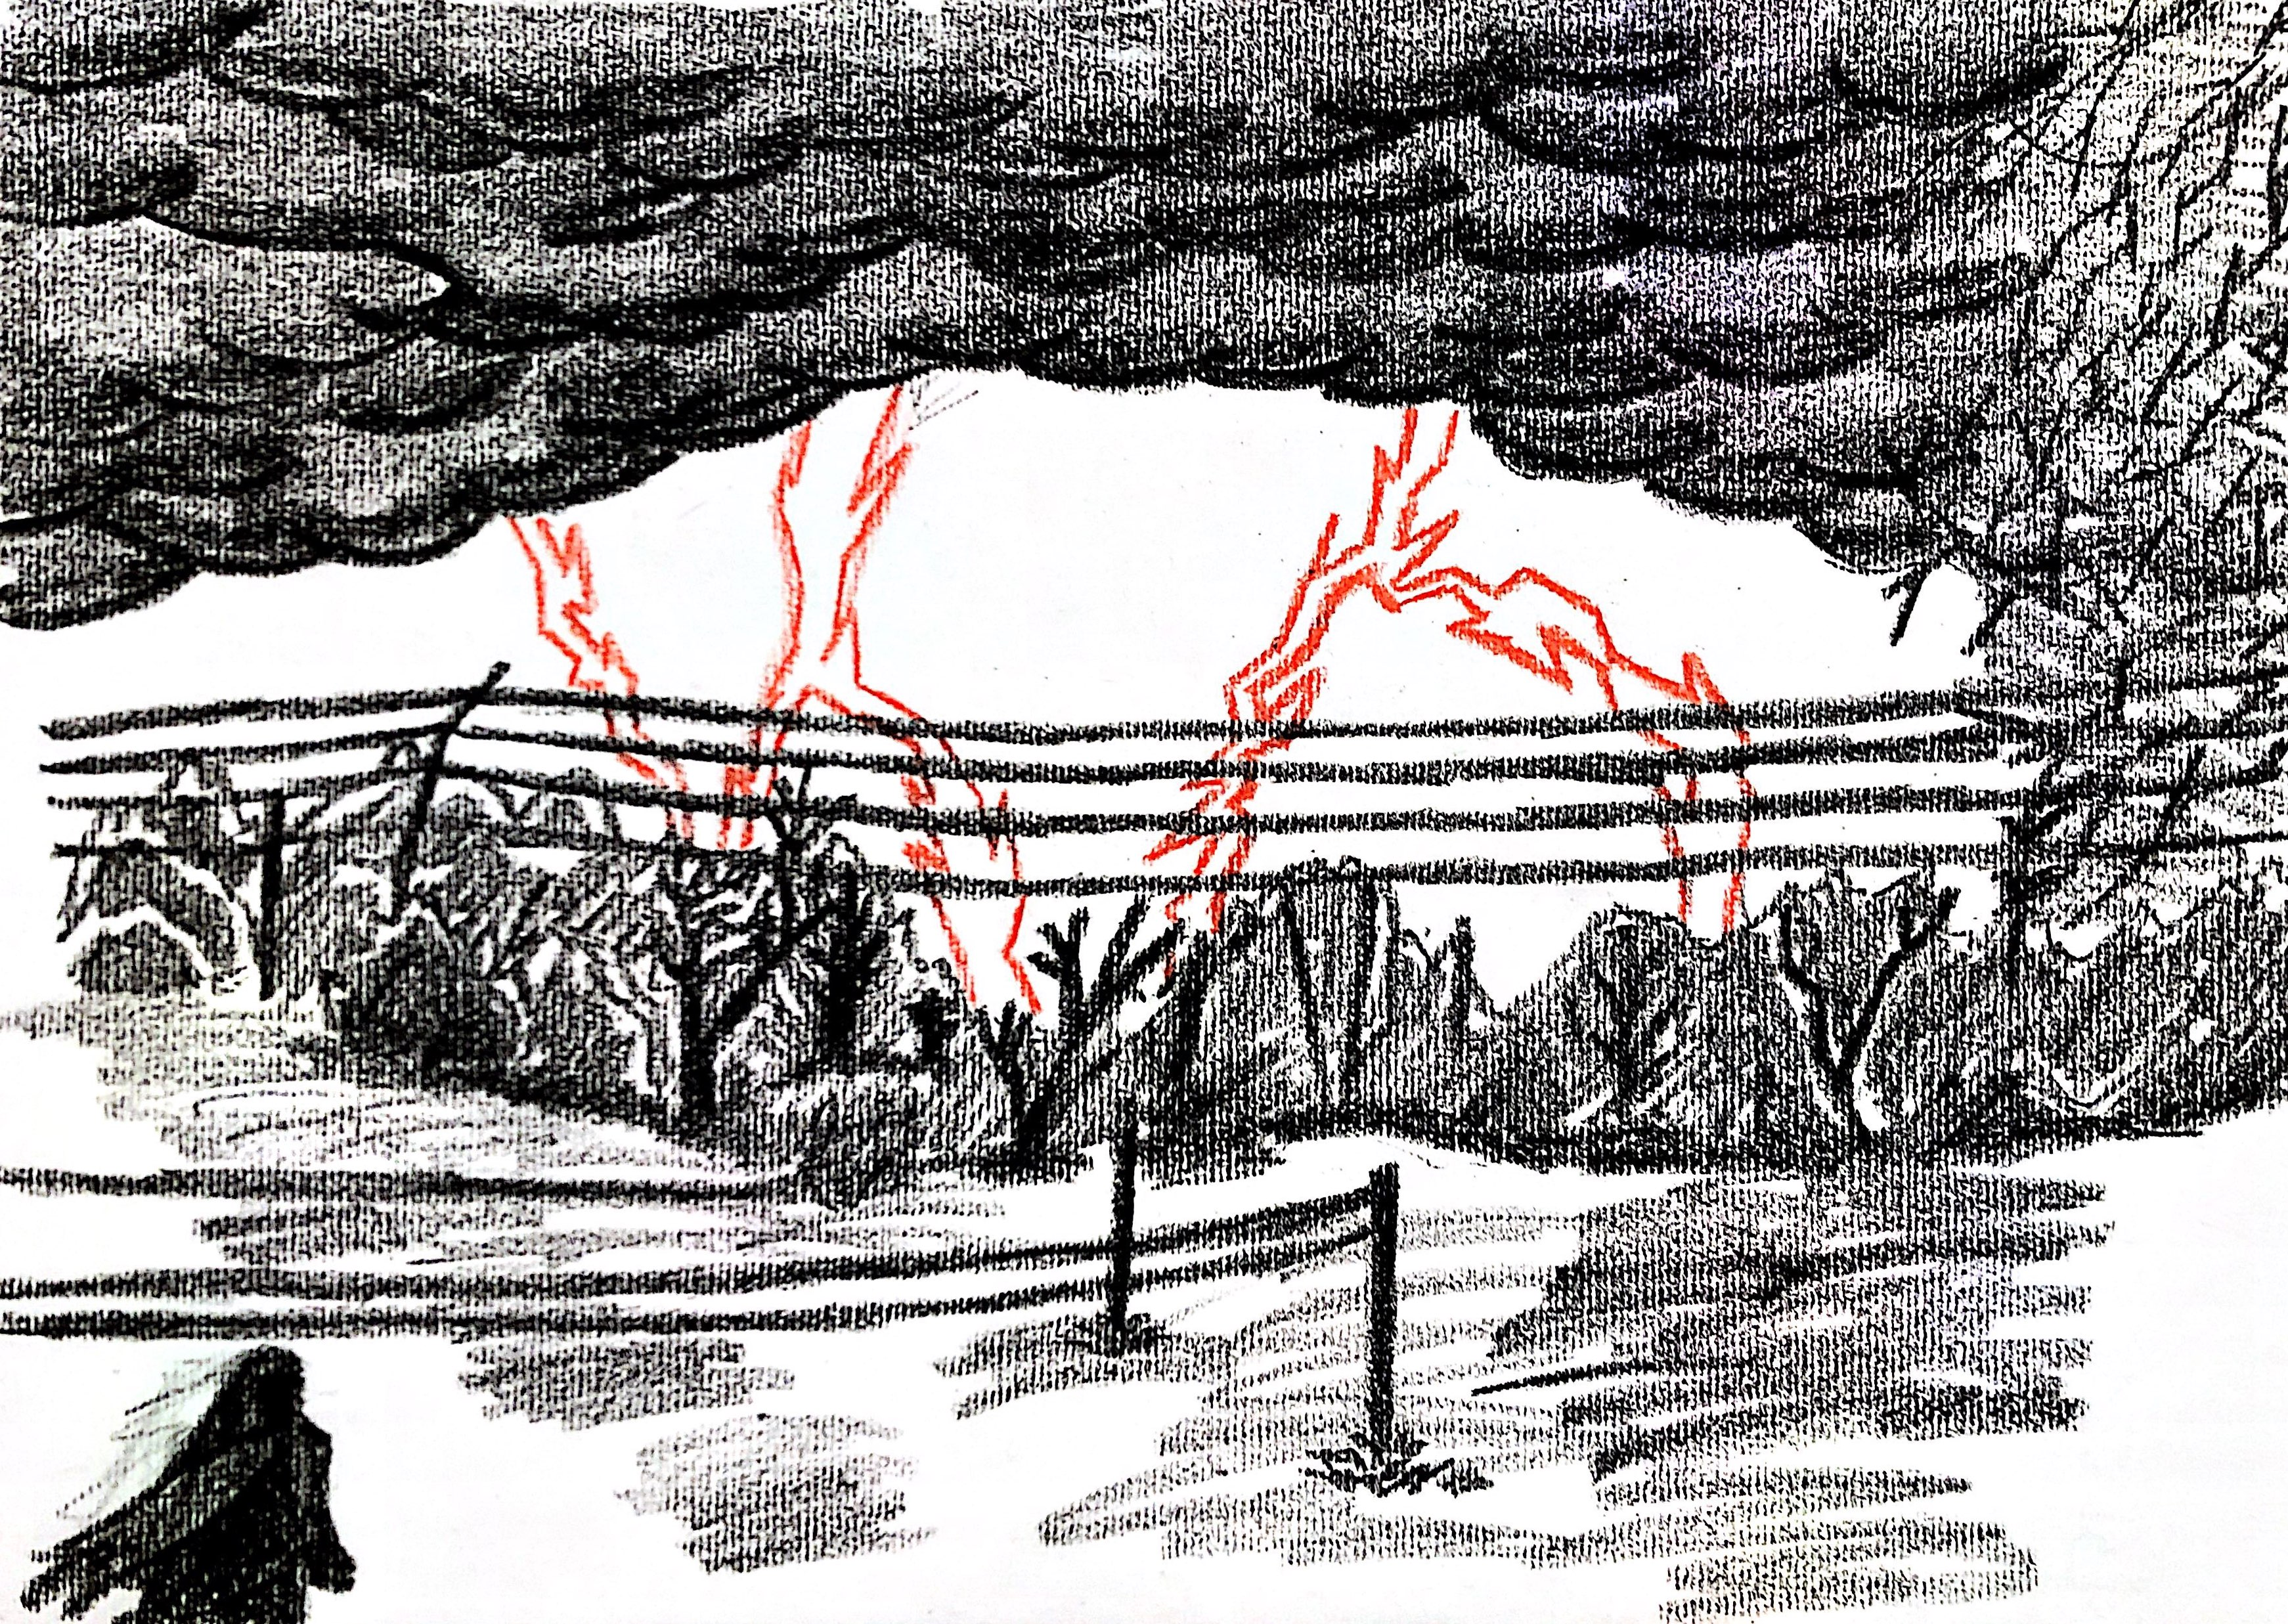
\includegraphics[width=15cm]{images/frontespizio/cover.jpg}
	\end{center}

	\vspace*{7mm}

	\begin{center}
		\LARGE DEMON PARTY\\
		\vspace*{2mm}
		\Large Game and Level Design\\
		\large Academic Year 2019/2020
	\end{center}

	\newpage

	\begin{figure}[H]
		\centering
		
\includegraphics[width=0.8\linewidth]{images/frontespizio/demonparty_logo.jpg}
	\end{figure}

	\vspace*{2mm}

	\begin{center}
		\textbf{Gerard Baholli}\\
		\textit{943594} - \texttt{gerard.baholli@studenti.unimi.it}\\
		
		\vspace*{7mm}
		
		\textbf{Edoardo D'Angelo}\\
		\textit{947729} - \texttt{edoardo.dangelo1@studenti.unimi.it}\\
		
		\vspace*{7mm}
		
		\textbf{Mihail Moraitis}\\
		\textit{953609} - \texttt{mihail.moraitis@studenti.unimi.it}\\
	\end{center}

}

\thispagestyle{empty}

	\begin{center}
		\begin{tabular}[c]{| p{3cm} | p{3cm} | p{8cm} |}
			\hline
			\multicolumn{3}{| c |}{\textbf{Revision History}}\\
			\hline\hline
			\textbf{Who} & \textbf{Date}  & \textbf{Comment}\\
			\hline
			Gerard Baholli & 03/11/2019 & Creation of this document\\
			\hline
			Edoardo D'Angelo & 05/11/2019 & Added high concept\\
			\hline
			Gerard Baholli & 05/11/2019 & Added world diagram\\
			\hline
			Mihail Moraitis & 05/11/2019 & Added goals outline\\
			\hline
			Edoardo D'Angelo & 06/11/2019 & Added synopsis\\
			\hline
			Mihail Moraitis & 06/11/2019 & Updated goals outline\\
			\hline
			Gerard Baholli & 07/11/2019 & Added graphs, first milestone revision\\
			\hline
			Edoardo D'Angelo & 11/11/2019 & Story updated\\
			\hline
			Gerard Baholli & 14/11/2019 & Goals outline review\\
			\hline
			Mihail Moraitis & 21/11/2019 & Updated world diagram\\
			\hline
			Edoardo D'Angelo & 25/11/2019 & Added level design dialogues\\
			\hline
			Gerard Baholli & 26/11/2019 & Added graphs\\
			\hline
			Mihail Moraitis & 27/11/2019 & Added periodic table\\
			\hline
			Edoardo D'Angelo & 28/11/2019 & Second milestone review\\
			\hline
			Edoardo D'Angelo & 01/11/2019 & Level description updated\\
			\hline
			Gerard Baholli & 02/11/2019 & Added enemies\\
			\hline
			Mihail Moraitis & 04/11/2019 & Added skill chart and enemy chart\\
			\hline
			Mihail Moraitis & 08/11/2019 & Enemies review\\
			\hline
			Mihail Moraitis & 09/11/2019 & Added scope\\
			\hline
			Gerard Baholli & 10/11/2019 & Skill chart and enemy chart review\\
			\hline
			Edoardo D'Angelo & 12/11/2019 & Third milestone review\\
			\hline
			Gerard Baholli & 26/11/2019 & Added graphs\\
			\hline
			Mihail Moraitis & 27/11/2019 & Added periodic table\\
			\hline
			Edoardo D'Angelo & 28/11/2019 & Second milestone review\\
			\hline
			Edoardo D'Angelo & 01/12/2019 & Level description updated\\
			\hline
			Gerard Baholli & 02/12/2019 & Added enemies\\
			\hline
			Mihail Moraitis & 04/12/2019 & Added skill chart and enemy chart\\
			\hline
			Mihail Moraitis & 08/12/2019 & Enemies review\\
			\hline
			Mihail Moraitis & 09/12/2019 & Added scope\\
			\hline
			Gerard Baholli & 10/12/2019 & Skill chart and enemy chart review\\
			\hline
			Edoardo D'Angelo & 12/12/2019 & Third milestone review\\
			\hline
			
			Gerard Baholli & 26/12/2019 & Added characters\\
			\hline
			Mihail Moraitis & 27/12/2019 & Added fight outcomes\\
			\hline
			Edoardo D'Angelo & 28/12/2019 & Review goals outline\\
			\hline
			Edoardo D'Angelo & 01/01/2020 & Level description updated\\
			\hline
			Gerard Baholli & 02/01/2020 & Review enemies chart and level diagram\\
			\hline
			Mihail Moraitis & 04/01/2020 & Added periodic table\\
			\hline
			Mihail Moraitis & 08/01/2020 & Enemies review\\
			\hline
			Mihail Moraitis & 09/01/2020 & Added scope\\
			\hline
			Edoardo D'Angelo & 12/01/2020 & Added additional mechanics\\
			\hline
			Gerard Baholli & 10/01/2020 & Review additional mechanics\\
			\hline
			Gerard Baholli & 11/01/2020 & Added level map\\
			\hline
			Edoardo D'Angelo & 12/01/2020 & Added event diagram and level diagram\\
			\hline
			Mihail Moraitis & 13/01/2020 & Added puzzles\\
			\hline
			Edoardo D'Angelo & 15/01/2020 & Review fights\\
			\hline
			Gerard Baholli & 16/01/2020 & Review map measures\\
			\hline
			Edoardo D'Angelo & 17/01/2020 & Final review\\
			\hline
		\end{tabular}
	\end{center}
	

\tableofcontents

\section{High Concept}

\subsection{Game}

This is a single player adventure game, mainly focused on storytelling, exploration and real time combat. The player's avatar is a twisted version of the
main character of Stranger Things: Eleven. This copy has the same memories as the original, so at the starting point they are identical.
The game has, in addition to the main combat system, two main features:

\begin{itemize}
	\item After a certain level, you can use demons to explore new areas that can only be reached through a mini-game.
	\item During the adventure, the player will be accompanied by several NPCs who will be able to give active and passive support.
\end{itemize}

Lastly, during boss battles, it will be possible to interact with some elements of the map that can change the flow of the fight, such as giving buffs, malus or damage.

\subsection{Story}
The story stars BAD Eleven, a copy of Eleven, looking for a way to leave the Upside Down. After learning the basic techniques of survival from a mysterious man named Kyle, Elby will undertake a journey in search of the Numbers, people on whom experiments have been conducted, just like his original counterpart. Each of these people has special abilities, which led them to have different survival methods and goals. They will therefore be described the rules behind the Upside Down and the events that will lead it to a radical change.
\section{Settings/Fundamental concepts}
The story is set in the Upside-Down, a dimension parallel to ours, in which there is little light and everything is covered with organic matter.
The starting point is Hawkins, a small town in Texas, where there is a school and a library. The city is surrounded by a forest, called Mirkwood, at the center of which is the energy laboratory, connected by drains to Lake Hawkins. Crossing the Old Sabine Wildlife you can reach Lindale, home of the museum. Far more distant is instead Dallas, the only fortified city not covered by organic matter. Finally, using an underground tunnel, you reach Fort Worth, now in ruins and a creature's lair.

The following laws, theories and concepts that govern the dimension of the Upside-Down will be explained by characters and/or documents within the game.

\begin{itemize}
	\item Time and Space: The Upside-Down is an alternative dimension that has the same characteristics and the same physical structures as our reality, but covered with organic material. It is therefore possible to hypothesize that this mass is produced by an organism that extends over an extremely large area, if not all over the globe. This non-sentient creature, called Upside-Down Core, has the Chronokinesis, a skill that allows it to replicate the structure of our reality at a given instant of time and apply it to the Upside-Down. This process takes place with a fixed and 
	continuous cadence, but only in the areas in which its organic matter extends.
	\item Dimensional Travel: when a person with high kinetic abilities abuses his power, there is the possibility that he does not die but is transported to the Upside Down. Here, with the exception of fortuitous cases or particular abilities, it remains trapped there without the possibility of escape.
	\item Demons: Except for the DemoGorgon with which Eleven had come into contact, no other demon has the ability to open gaps between dimensions.
\end{itemize}


\section{Themes}
\textbf{What is right and what is wrong}\\
Motivations and actions of the various characters are always analyzed from different points of view, questioning whether they are right or wrong.\\\\
\textbf{Endless Isolation, Eternal Darkness}\\
Each character faces the solitude and desolation of the Upside-down in its own way, leading to different psychological evolutions.\\\\
\textbf{Oh, that's why...}\\
A fundamental point of the game is the explanation of the laws and / or properties of the upside-down. The player must be able to fill in the gaps of the
main series and understand why things have evolved in a certain way.

%
\section{Periodic Table of Storytelling }


\begin{center}
	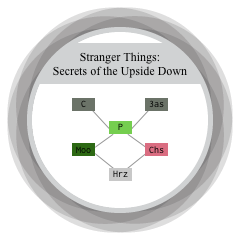
\includegraphics[width=0.75\linewidth]{images/story_molecolar.png}
\end{center}

\vspace*{2mm}

Description of the elements:\\
\textbf{\textcolor{LimeGreen}{[P]} Protagonist}: Bad Eleven is the protagonist of the story.\\
%\textbf{\textcolor{LimeGreen}{[A]} Antagonist}: Kyle, a powerful magician.\\
%\textbf{\textcolor{LimeGreen}{[Rnd]} Rounded Character​}: \#010 gradually loses her kind-hearted attitude during the story due to the death of her brother. In the end she will turn good again and feel guilty for the bad feelings harboring in her heart.\\
\textbf{\textcolor{dark-gray}{[3as]} Three Act Structure}: The story begins with a Setup act (introduction of characters setting and context), continues with a Confrontation and Evolution act (meeting with \#009 and \#010 encounters \#001) and ends with a Resolution act (after the final battle the protagonist ends his evolution).\\
%\textbf{\textcolor{dark-gray}{[Cmx]} The Climax}: The final battle is the most important event in the story, involving directly and indirectly every characters.\\
\textbf{\textcolor{dark-gray}{[C]} Conflict}: Kyle has a plan to control the Upside-Down Core and he kills \#005 and \#010 for this purpose. Elby will stop him with \#009 help, who is looking for revenge.\\
\textbf{\textcolor{OliveGreen}{[Moo]} Mooks}: The standard enemies, like Demonrats and Demondogs.\\
\textbf{\textcolor{Salmon}{[Chs]} The Chessmaster}: Kyle gets the name of chessmaster from his ability to manipulate events. he uses the protagonist to obtain informations about the numbers and uses them as if they were pieces on a chessboard.\\
\textbf{\textcolor{light-gray}{[Hrz]} Moral Event Horizon}: After the end of the Act II, Kyle'll have a mental breakdown and will become like a mindless man seeking only destruction. From that moment he will be pure evil.\\
\section{Synopsis}

The death of the DemoGorgon, killed by Eleven, starts a paradox that, in addition to carrying the girl in the Upside-down, generates a reincarnation of 
the demon in the form of El herself, called B.A.D. Eleven (Biological Altered Demon \#011), having the same memories and abilities as the original.

\subsection{Act I}
BAD Eleven (Elby for short) wakes up in Hawkins school, confused and scared. Wandering through the building, he sees Eleven escaping through a portal, 
but later, after trying to get in, discovers that she can't cross it. After having faced a Demon generated by the remains of Barbara's body in the library, she meets in the courtyard Blank, a survivor of the Upside-Down, who leads her to his shelter. Here, after having taught her the basics of survival, he suggests that she should go to the laboratory to escape from the Upside-Down through the portal opened by Eleven. Elby then walks towards the structure, but once she reaches the gap, she again fails to cross it. While heading for the exit,she finds the data and photos of projects \#003, \#005 and \#009. Back at the shelter, she uses her telekinesis to locate the three numbers and decides to go looking for \#005, while Blank will meet \#003.\\

\{To be defined\} (Journey to Lindale, meet with \# 005)\\

Elby and \#005 return to the shelter, where he begins to become suspicious of the identity of Blank. Having no further clues about the portal 
crossing method, they decide to leave for Dallas to meet \#009. Meanwhile Blank managed to find \#003.

\subsection{Act II}
\{To be defined\} (Arrival in Dallas, Introduction of \#009 and \#010, Reveal of Blank into \#001, Abduction of \#005)\\

Reached the Upside-Down Core, Elby and \#010 are captured by \#001 and assist while he kills \#005 and extracts its powers through the use of a parasite. 
Having now both the biocynesis and the mental synchronization with the demons, \#001 is able to take control of the Core and use its chronocynesis at will.
Threatening to kill \#010, he forces Elby to open a portal, thus completing his plan to return home in the time instant he craves. However, it is revealed
that this is another alternative reality, and that it is therefore impossible to recreate the conditions to have the correct time and space. This causes a 
psychological breakdown in \#001, which kills \#010 and uses its powers to create a giant creature for the purpose of transporting the Core and expanding 
the Upside-Down to all realities, starting with that he came from.

\subsection{Act III}
\{To be defined\} (Dallas Resistance, Creature Defeat, Final Battle)\\

After the final battle, which foresees the death of all the surviving numbers, it is possible to see the Upside-Down Core, still active, while incorporating
the corpses of \#001 and BAD \#011. This causes a mutation in the creature, which takes shape of a giant spider and becomes a sentient entity, later called 
Mind Flayer. Reference is therefore made to the will of the demon to invade other dimensions (influence of \#001) and to the hatred it feels towards Eleven 
(influence of BAD \#011), characteristics seen in the Second and Third Season.

\section{Story Flowchart}

\vspace*{0.5cm}
\begin{center}
	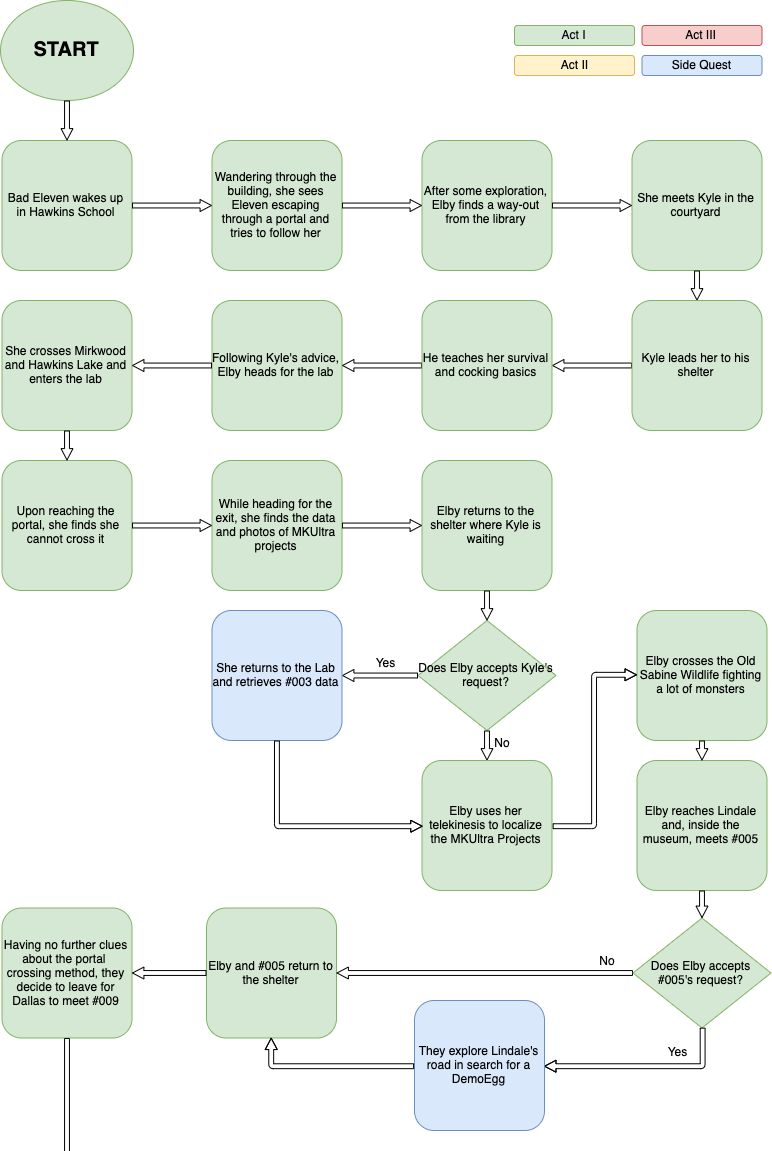
\includegraphics[width=0.99\linewidth]{images/graphs/story_flowchart_1.png}
\end{center}


\begin{center}
	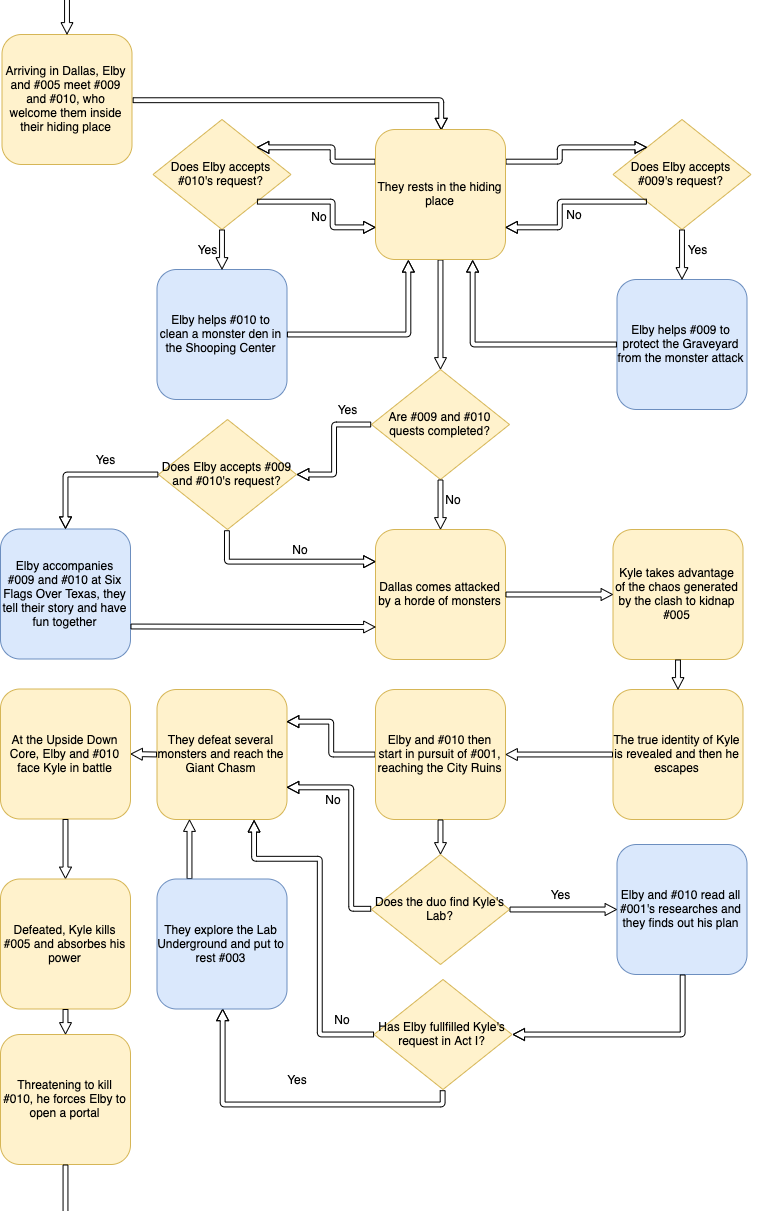
\includegraphics[width=0.99\linewidth]{images/graphs/story_flowchart_2.png}
\end{center}



\begin{center}
	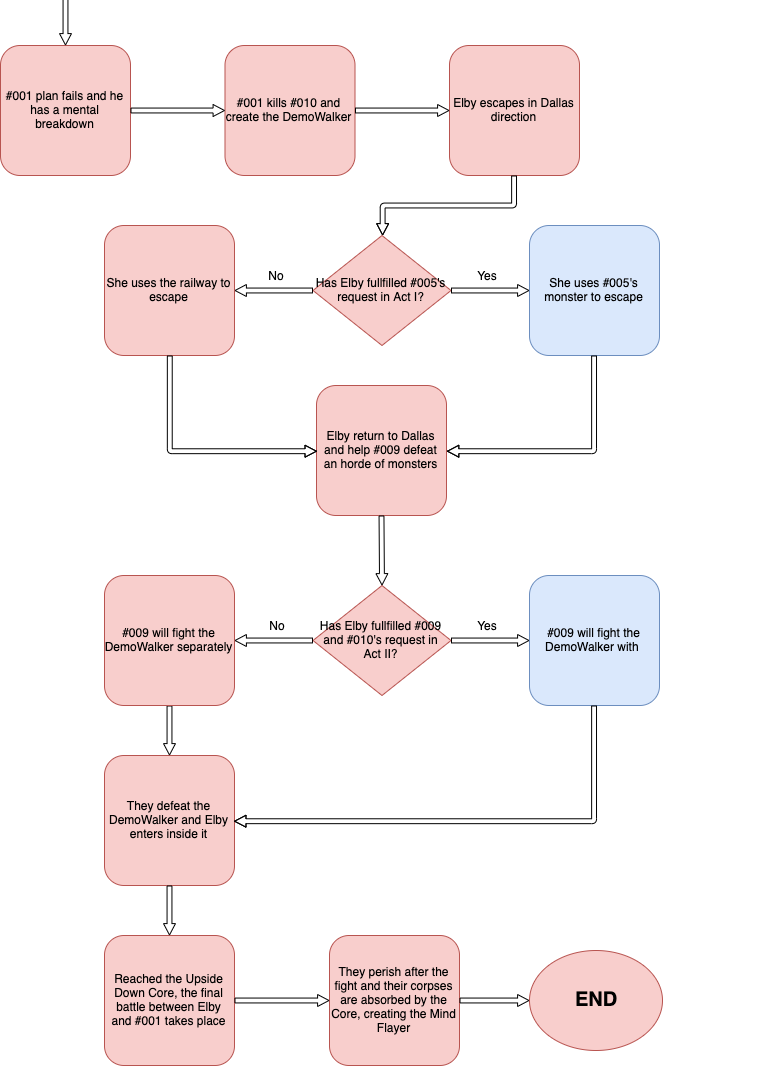
\includegraphics[width=0.99\linewidth]{images/graphs/story_flowchart_3.png}
\end{center}
\section{World Diagram}

\vspace*{1cm}
\begin{center}
	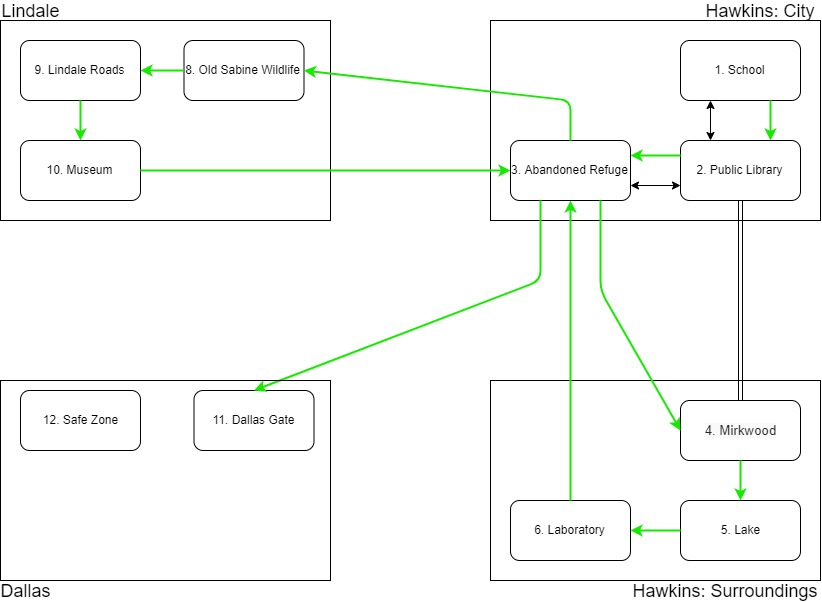
\includegraphics[width=0.8\linewidth]{images/graphs/worlddiagram.jpg}
\end{center}
\section{Goals Outline}

\subsection{Hawkins: City}
\begin{itemize}
	\item Real World: Dream
	\begin{itemize}
		\item Tutorial
	\end{itemize}
\end{itemize}
\begin{itemize}
	\item School
	\begin{itemize}
		\item Find the key of the door
		\item Look for the map
		\item Defete the rats
		\item Go to the point indicated in the map
	\end{itemize}
	\item Public Library
	\begin{itemize}
		\item Find the book
		\item Look for the map
		\item Defeat the Boss
		\item Go to the point indicated in the map
	\end{itemize}
	\item Abandoned Refuge
	\begin{itemize}
		\item Talk to Blank
		\item Survival tutorial
		\item Cooking tutorial
	\end{itemize}
\end{itemize}

\subsection{Hawkins: Surroundings}
\begin{itemize}
	\item Mirkwood
	\begin{itemize}
		\item Defeat the demons
		\item Craft a chain
		\item Look for the map
	\end{itemize}
	\item Lake
	\begin{itemize}
		\item Find a way to the lab
		\item Defeat the DemoLeviatan -Bob-
		\item --Find the One Piece Treasure--
	\end{itemize}
	\item Laboratory
	\begin{itemize}
		\item Find the elevator
		\item Find an alternative route
		\item Look for a way out
	\end{itemize}
\end{itemize}

\subsection{Lindale}
\begin{itemize}
	\item Old Sabine Wildlife
	\begin{itemize}
		\item Open a new path -puzzle-
		\item Look for food
		\item Defete the DemoSpiders
	\end{itemize}
	\item Lindale Roads
	\begin{itemize}	
		\item Find the key of the door
		\item Look for the map
		\item Defete the Demons
		\item Search for suits
		\item Look the journal
		\item Find a Rope
	\end{itemize}
	\item Museum
	\begin{itemize}
		\item Talk with \#005
		\item Find the backdoor
		\item Defeat the Boss
	\end{itemize}
\end{itemize}

\subsection{Dallas}
\begin{itemize}
	\item Road to Dallas
	\begin{itemize}	
		\item Complete the DemoDog minigame
	\end{itemize}
	\item Dallas Gate
	\begin{itemize}
		\item Talk with \#009 \#010
		\item Search for a way in
		\end{itemize}
	\item Station
	\begin{itemize}
		\item Clear the railroads
		\item Fortify the station
		\item Defete the dogs
		\item Find the gear -part 1-
	\end{itemize}
	\item Graveyard
	\begin{itemize}
		\item Speak with \#009
		\item Defete the DemonWorms
		\item Find the gear -part 2-
	\end{itemize}
\end{itemize}

\subsection{Core}
\begin{itemize}
		\item Road to the Core
		\begin{itemize}	
			\item Complete the DemoDog minigame
		\end{itemize}
	\item City Ruins
	\begin{itemize}
		\item Find the exit of the labirinth
		\item Open the laboratory of Blank
		\item Defeat the Demons
		\item Find the Suit
	\end{itemize}
	\item Laboratory Blank
	\begin{itemize}
		\item Complete the puzzle
		\item Kill the DemoParacites
		\item Destroy the lab
	\end{itemize}
	\item Core
	\begin{itemize}
		\item Defeat \#001
		\item Escape from the Core
	\end{itemize}
\end{itemize}

\subsection{Dallas -final-}
\begin{itemize}
		\item Return to Dallas
		\begin{itemize}	
			\item Complete the DemoDog minigame
		\end{itemize}
	\item War zone -Safezone-
	\begin{itemize}
	\item Help \#009
	\item Defeat the giant creature
	\end{itemize}
\end{itemize}
\subsection{Core -final-}
\begin{itemize}
	\item War zone -Safezone-
	\begin{itemize}
		\item Solve the puzzle
		\item Find the dungeon core
		\item Defeat \#001 
	\end{itemize}
\end{itemize}



\section{Scope}

\vspace*{0.5cm}

\begin{center}
	\begin{tabular}[c]{| p{6cm} | p{4cm} | p{3cm} |}
		\hline
		\textbf{Level} & \textbf{Estimated time} & \textbf{Percentage} \\
		\hline
		1. School & 20 minutes & 3\% \\
		\hline
		2. Public Library & 40 minutes & 7\% \\
		\hline
		3. Abandoned Refuge & 20 minutes & 3\% \\
		\hline
		4. Mirkwood & 25 minutes & 5\% \\
		\hline
		5. Lake & 45 minutes & 8\% \\
		\hline
		6. Laboratory & 25 minutes & 5\% \\
		\hline
		7. Abandoned Refuge & 25 minutes & 5\% \\
		\hline
		8. Old Sabine Wildlife & 40 minutes & 7\% \\
		\hline
		9. Lindale Roads & 25 minutes & 5\% \\
		\hline
		10. Museum & 25 minutes & 5\% \\
		\hline
		11. Dallas Gate & 50 minutes & 9\% \\
		\hline
		12. World Aquarium & 25 minutes & 5\% \\
		\hline
		13. Station & 25 minutes & 5\% \\
		\hline
		14. City Ruins & 25 minutes & 5\% \\
		\hline \rowcolor{light-light-gray}
		15. Giant Chasm & 60 minutes & 11\% \\
		\hline
		Ex. Shopping Center & 20 minutes & 3\% \\
		\hline
		Ex. Graveyard & 20 minutes & 3\% \\
		\hline
		Ex. Six Flags Over Texas & 20 minutes & 3\% \\
		\hline
		Ex. Lab Underground & 20 minutes & 3\% \\
		\hline \hline
		\textbf{Total Scope} & \textbf{9 hours 25 minutes} & \textbf{100\%} \\
		\hline
	\end{tabular}
\end{center}
\section{Enemy Chart}

\vspace*{0.2cm}

\subsection{Common}

\vspace*{0.2cm}

\begin{center}
	\begin{tabular}[c]{| p{2.4cm} | p{1cm} | p{1cm} | p{1cm} | p{1cm} | p{1.7cm} | p{1cm} | p{1.4cm} | p{1cm} | }
		\hline
		& Demo rats & Demo bats & Demo dog & Demo ants & Demo ants Queen & Demo wolves & Demo parasites & Demo moles \\
		\hline
		School & Yes & & & & & & &\\
		\hline
		Public Library & Yes & & & & & & &\\
		\hline
		Abandoned Refuge & Yes & & & & & & & \\
		\hline
		Mirkwood & Yes & & & & & & &\\
		\hline
		Lake & & & & & & & &\\
		\hline
		Laboratory & & & & & & & &\\
		\hline
		Abandoned Refuge & & & & & & & &\\
		\hline
		Old Sabine Wildlife & & & & & & & &\\
		\hline
		Lindale Roads & & & & & & & &\\
		\hline
 		Museum & & & & & & & &\\
		\hline
		Dallas Gate & & & & & & & &\\
		\hline
		World Aquarium & & & & & & & &\\
		\hline
		Station & & & & & & & &\\
		\hline
		City Ruins & & & & & & & &\\
		\hline \rowcolor{light-light-gray}
		Giant Chasm & Yes & & & & & & &\\
		\hline
		Shopping Center & & & & & & & &\\
		\hline
		Graveyard & & & & & & & &\\
		\hline
		Six Flags Over Texas & & & & & & & &\\
		\hline
		Ex. Lab Underground & & & & & & & &\\
		\hline
	\end{tabular}
\end{center}

\vspace*{0.2cm}

*Our level is underlinded in gray color.

\newpage

\subsection{Boss}

\vspace*{0.2cm}

\begin{center}
	\begin{tabular}[c]{| p{2.4cm} | p{1.5cm} | p{1.5cm} | p{1.5cm} | p{1.5cm} | p{1.5cm} | p{1.5cm} |}
		\hline
		& Demo Barbara & Demo leviathan & Demo nemesis & Demo walker & Demo cerberus & \#011 \\
		\hline
		School & & & Yes & & & \\
		\hline
		Public Library & Yes & & & & & \\
		\hline
		Abandoned Refuge & & & & & & \\
		\hline
		Mirkwood & & & & & & \\
		\hline
		Lake & & Yes & & & & \\
		\hline
		Laboratory & & & & & & \\
		\hline
		Abandoned Refuge & & & & & & \\
		\hline
		Old Sabine Wildlife & & & & & & Yes \\
		\hline
		Lindale Roads & & & & & & \\
		\hline
		Museum & & & & & & \\
		\hline
		Dallas Gate & & & Yes & & & \\
		\hline
		World Aquarium & & & & & & \\
		\hline
		Station & & & & & & \\
		\hline
		City Ruins & & & & & & \\
		\hline \rowcolor{light-light-gray}
		Giant Chasm & & & & & Yes & \\
		\hline
		Shopping Center & & & & & & \\
		\hline
		Graveyard & & & & & & \\
		\hline
		Six Flags Over Texas & & & & & & \\
		\hline
		Ex. Lab Underground & & & & & & \\
		\hline
	\end{tabular}
\end{center}

\vspace*{0.2cm}

*Our level is underlinded in gray color.

\section{Skill Chart}

\vspace*{0.5cm}

\begin{center}
	\begin{tabular}[c]{| p{3cm} | p{1.2cm} | p{1.2cm} | p{1.2cm} | p{6cm} |}
		\hline
		& Damage & Area & Range & Description \\
		\hline
		Focus & - & - & - & Regenerate 6 mana or give 1d4 bonus damage to the next hit.\\
		\hline
		Psicohit & 2d4 & 1 & 3m & This is a small hit that Bad Eleven uses to hit small enemies.\\
		\hline
		Barrier & 1d4 & 1 & - & This spell is a simple barrier that blocks a small ammount of damage.\\
		\hline
		Repel & 3d6 & - & - & This spell is a strong barrier that blocks half of the damage received and repel 3d6 to the enemy.\\
		\hline
		Psicochain & 1d4 & 1 & 3m & This is a stun that blocks 1 enemy for 1 or 2 turns.\\
		\hline
		Psicoslash & 2d6 & 1x3 & 5m & Bad Eleven hits the enemy with a mental sword.\\
		\hline
		Psicobeam & 5d6 & 10x1 & 10m & The distance is a strong factor in the game so Bad Eleven hit the enemy with a beam.\\
		\hline
		Psicobomb & 3d12 & 3x3 & 8m & This spell can hit more enemies at a time and slows them by 20\%.\\
		\hline
		Mastermind & - & - & - & It's a passive ability that regenerate 2 mana and give 2 bonus damage per turn.\\
		\hline
		Psicopush & 1 & 1 & 1m & Pushes the object or the enemy 2 meters away.\\
		\hline
	\end{tabular}
\end{center}
\section{Characters}

\subsection{B.A.D. Eleven}

\begin{wrapfigure}{l}{0.5\linewidth}
	\centering
	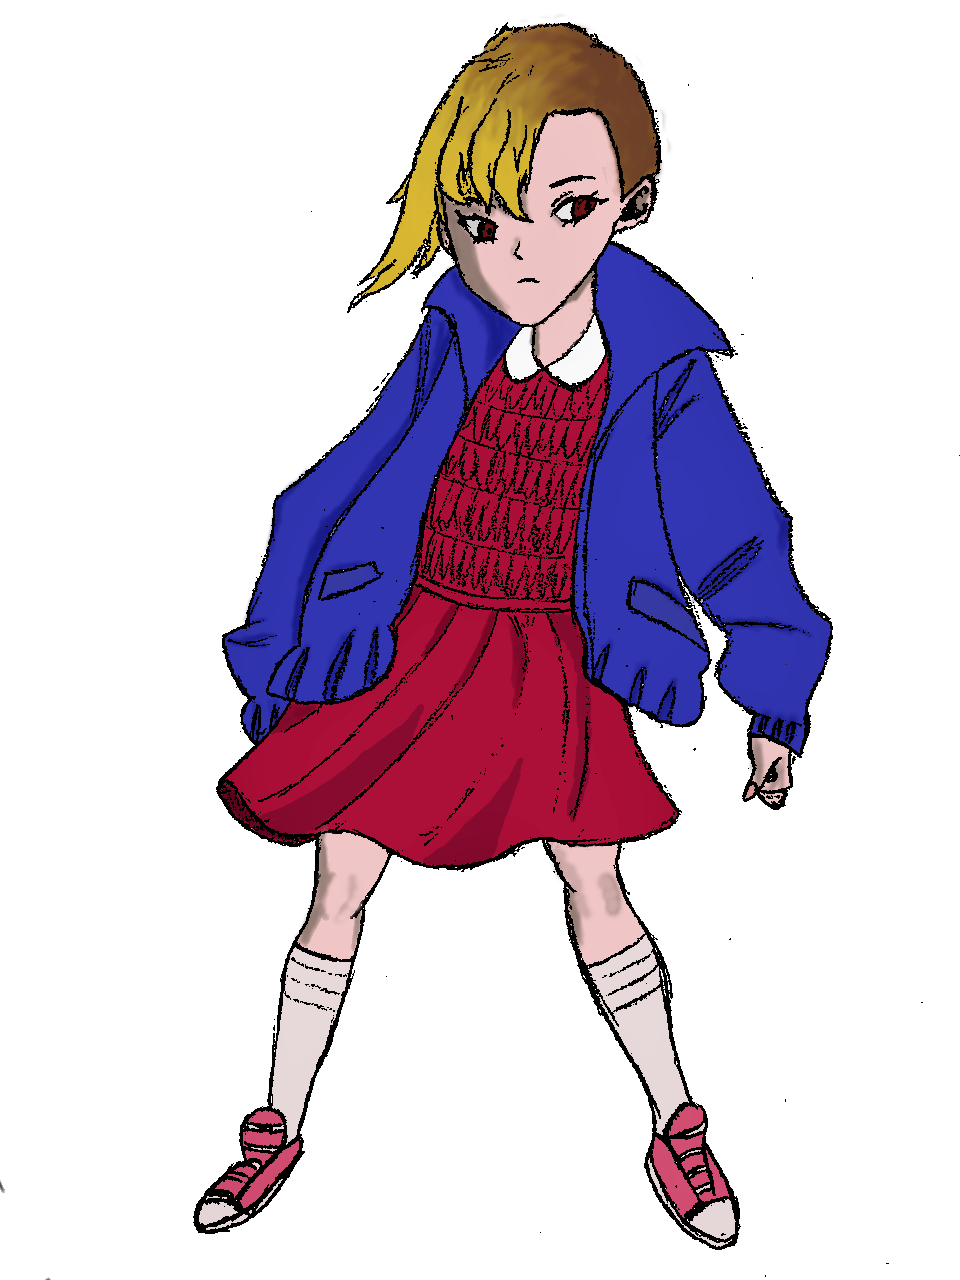
\includegraphics[width=0.5\linewidth]{images/characters/bad_eleven.png}
\end{wrapfigure}

Copy in everything of Eleven, BAD Eleven (Biological Altered Demon \#011, Elby) initially shares with her physical appearance, memories and attitudes. However, during the course of the story, it will be increasingly evident that, unlike the original, Elby cannot manage her emotions, for example by transforming "her" love for Mike and the desire to see him again in pure obsession. This will lead her to be apathetic and unscrupulous, ready to eliminate any obstacle between her and her escape. Contrary to heroic protagonists fueled by a need to help others and pursue good-intention motives that involve enacting the moral kind of justice, Elby's rogue path opts for a more personal and less moral kind of justice. She has the same telekinetic prowess as Eleven, but the side effect is greatly reduced and the development of her ability is clearly superior, probably due to the influence of the Upside-Down and her origins.

\vspace*{0.5cm}

%\subsubsection{Skills}

\subsubsection{Circumplex}
\begin{center}
	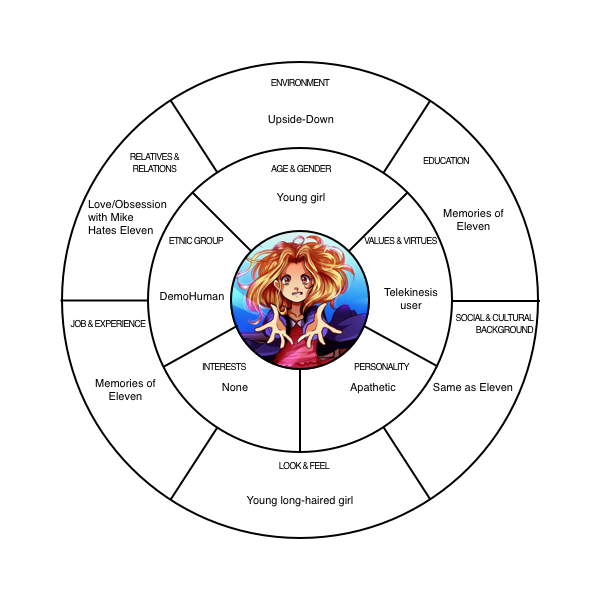
\includegraphics[width=0.76\linewidth]{images/circumplex/bad_eleven_circumplex.png}
	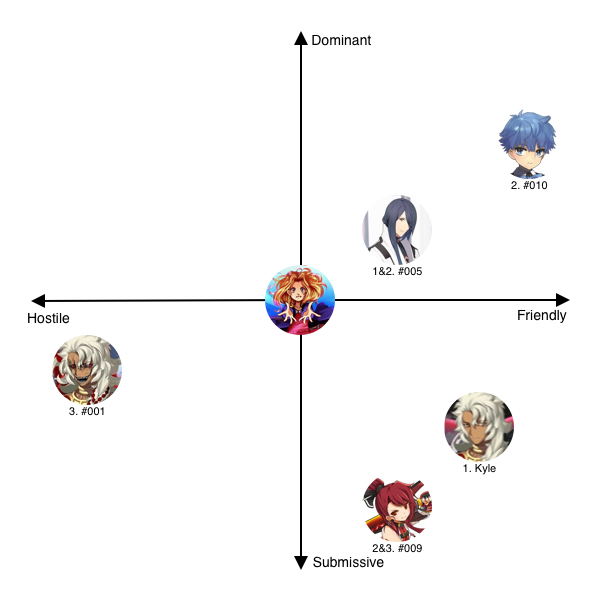
\includegraphics[width=0.76\linewidth]{images/map_of_relations/bad_eleven_map_of_relations.png}
\end{center}

\subsection{Kyle}

\begin{wrapfigure}{l}{0.5\linewidth}
	\centering
	
\includegraphics[width=0.8\linewidth]{images/characters/kyle_01.png}
	\caption{\textit{"Kyle first appearance [Artwork from Fate Grand Order]"}}
\end{wrapfigure}

Kyle, alias \#001, is the first experimental subject of the MKUltra project. He's a 29-year-old boy, trapped in the Upside-Down since he was 15.
Despite the friendly and gentle attitude, the long period spent in darkness and solitude has greatly affected his mental stability, making him bipolar 
and easily irritated. Since birth he has the mental ability of biocynesis, the control and manipulation over organic matter. This ability applied to the 
Upside-Down allows him to control the ramifications of the Upside-Down Core, on condition that he is quite far from it.
His goal is to return home, not in the present time, but when he was kidnapped for experimentation, so that he could regain life and happiness denied to him.
To do this he requires the temporal ability of the Core and Elby's telecynesis to open the gap.
His personality changes drastically after discovering that, due to the laws of the multiverse, his plan is destined to fail. It therefore becomes extremely violent and sadistic, not even sparing the other numbers, which he believes are destined to suffer and need to be released through death. Moreover, he decides
 to transport the Core in various dimensions, in order to expand the Upside-Down and make all the inhabitants of the alternate realities suffer the same torture imposed on him.

\subsubsection{Backstory}
Born in a quiet Texas town, Kyle lives a happy and carefree life with his family. At the age of 6 he began to show the first signs of biocynesis, succeeding in bringing back a withered flower. Initially the use of his ability caused him violent migraines, but the more years passed and he became stronger, the less the side effects were intense. Although his ability had been kept as secret as possible, at the age of 12 he was tracked down by Brenner and, after witnessing the massacre of his family, he was imprisoned in an experimentation facility. In addition to continuous blood withdrawals, necessary for the creation of a serum to be used for the artificial production of test subjects, he was forced to use the biocynesis for war purposes, until the day when, exceeding the limit of his ability to attempt a escape, he was wrapped in a black cloud and disappeared.

\subsubsection{Circumplex}
\begin{center}
	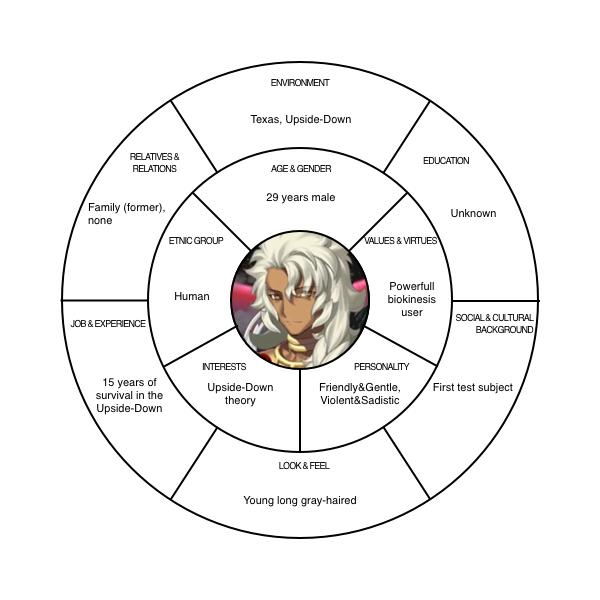
\includegraphics[width=0.76\linewidth]{images/circumplex/kyle_circumplex.png}
	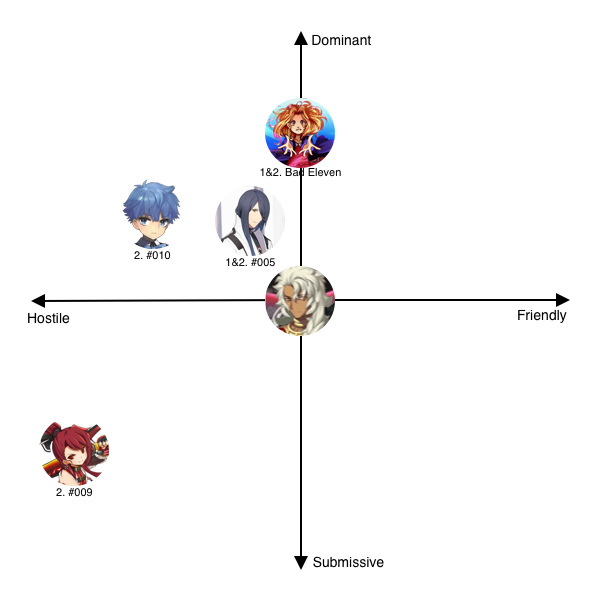
\includegraphics[width=0.76\linewidth]{images/map_of_relations/kyle_map_of_relations.png}
	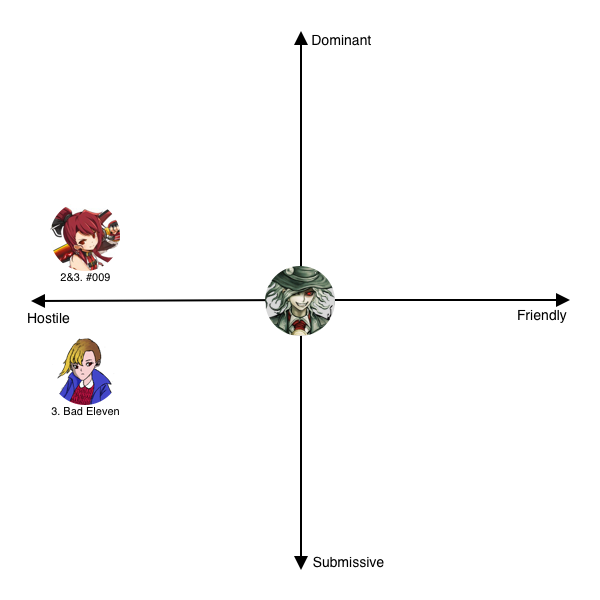
\includegraphics[width=0.76\linewidth]{images/map_of_relations/001_map_of_relations.png}
\end{center}

\newpage

\subsection{Minor characters}

\subsubsection{\#005}

\begin{wrapfigure}{l}{0.3\linewidth}
	\centering
	
\includegraphics[width=0.55\linewidth]{images/characters/005.png}
\end{wrapfigure}

\#005 is the fifth experimental topic of the MKUltra project. Together with \#003, he is part of the first generation of test subjects on which the serum produced by Kyle's blood was tested. \#005 does not appreciate the company of other people and prefers to spend his life in the Upside Down on his own, reading the few books he has found. Thanks to his ability, the Kinesis mental synchronization is able to partially control the monsters, keeping them away from his hiding place.\\


\subsubsection{\#009 and \#010}

\begin{wrapfigure}{l}{0.2\linewidth}
	\centering
	
\includegraphics[width=0.5\linewidth]{images/characters/009.png}
\end{wrapfigure}

Sister and brother, \#009 and \#010 are part of the second generation of test subjects on which serum from Kyle's blood was tested. While \#009 is a very strong and passionate girl, so comfortable in the Upside-Down that she calls herself the Queen of the same, \#010 is a very shy guy, always hiding in the shadow of her older sister.\\

\begin{wrapfigure}{l}{0.2\linewidth}
	\centering
	
\includegraphics[width=0.5\linewidth]{images/characters/010.png}
\end{wrapfigure}

Despite the difference in character, the two rarely separate and collaborate to survive in their new "home". \#009 prowess is the Pyrokinesis, the ability to accelerate atoms and create fire, while \#010 has the Cryokinesis, the ability to slow atoms and freeze things.\\


\subsubsection{Extra - \#003}

\begin{wrapfigure}{l}{0.3\linewidth}
	\centering
	
\includegraphics[width=0.55\linewidth]{images/characters/003.png}
\end{wrapfigure}

If the player completes Kyle's side quest and enters his lab, Elby will find secret documents containing \#003 data, in particular on the moment of her arrival in the Upside-Down and her prowess, Healing. In the basement of the laboratory it is possible to put to rest \#003 dead body, controlled and deformed by the experiments on her carried out by Kyle.

\section{Level Design}
In this section the sequences of the implemented level "Giant Chasm" are explained. The level is divided into 5 sequences.\\
Under the representative map of the section are listed all the dialogues belonging to that specific time section.

\subsection{Scope of the level}

\vspace*{0.5cm}

\begin{center}
	\begin{tabular}[c]{| p{6cm} | p{4cm} | p{3cm} |}
		\hline
		Section 1 &                & \\
		 - Entrance                   & 5 minutes                  & 8,33\%                 \\
		 - Democerberus Boss Room          & 10 minutes                  & 16,66\%                 \\
		 - External Ovest Side           & 5 minutes			                & 8,33\%	                  \\ \hline
		 Section 2 &                & \\
		 - Entrance                   & 2 minutes                  & 3,33\%                 \\
		 - Democerberus Boss Room          & 8 minutes                  & 13,33\%                 \\
		 - External Ovest Side           & 5 minutes		                & 8,33\%                  \\ \hline
		 Section 3 &                & \\
		 - Entrance                   & 5 minutes                  & 8,33\%                 \\
		 - Democerberus Boss Room          & 5 minutes                  & 8,33\%                 \\
		 - External Ovest Side           & 5 minutes			                & 8,33\%	                  \\ \hline
		 Final Boss Room           & 10	minutes		                & 16,66\%	                  \\ \hline
		 \textbf{Total Scope}              & \textbf{60 minutes} & \textbf{100\%}      \\ \hline
	\end{tabular}
\end{center}

*We only consider the playing time and not the dialogues (except for the final Boss).\\


\subsection{Event Diagram}

\begin{figure}[H]
	\centering
	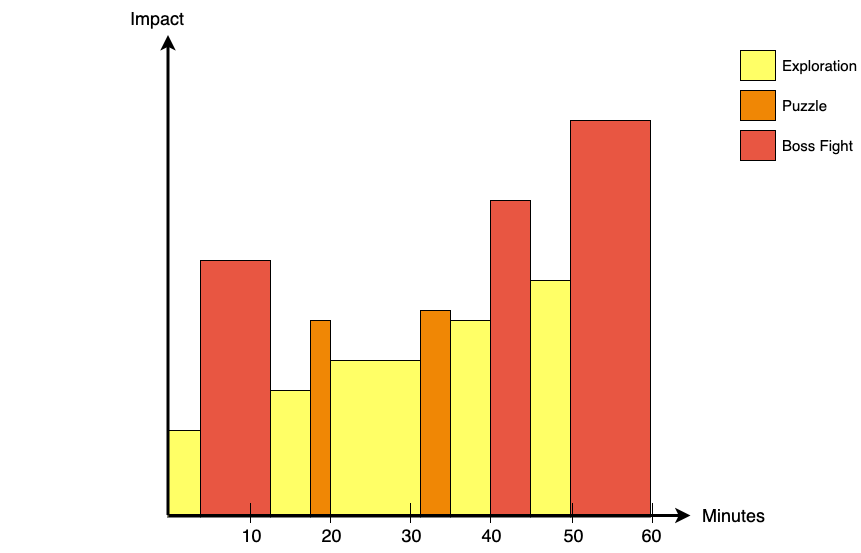
\includegraphics[width=0.8\linewidth]{images/graphs/event_diagram.png}
\end{figure}

\subsection{Level Map}

\begin{figure}[H]
	\centering
	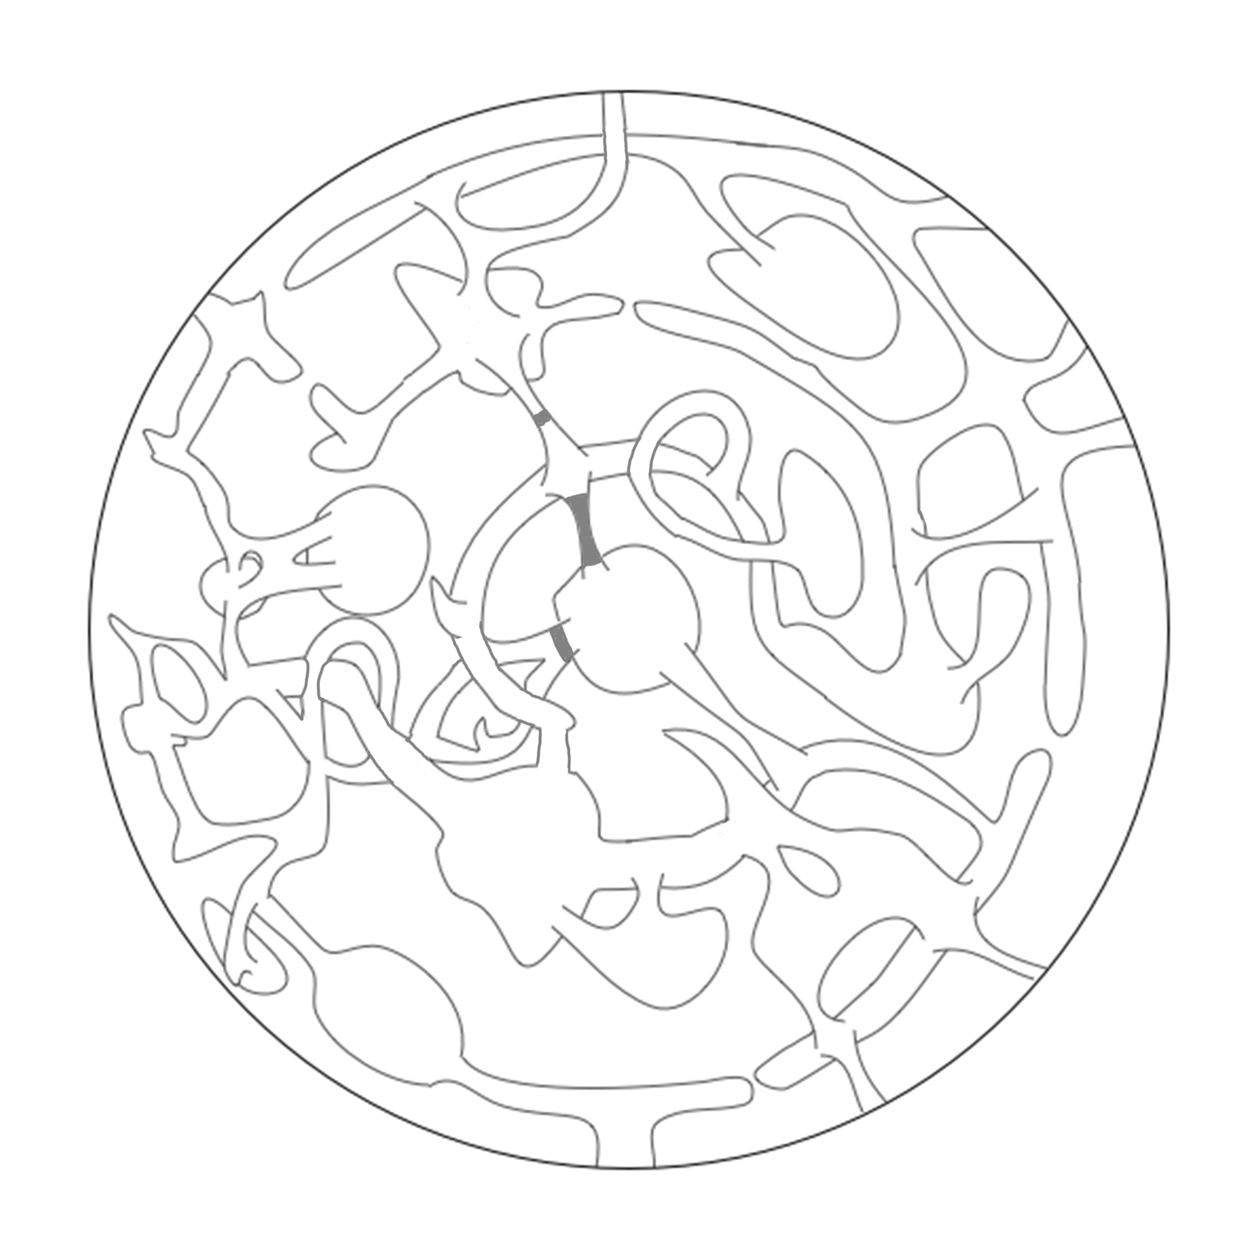
\includegraphics[width=0.6\linewidth]{images/map/map_clear.png}
	\caption*{Complete 2D map of the level}
\end{figure}

\begin{figure}[H]
	\centering
	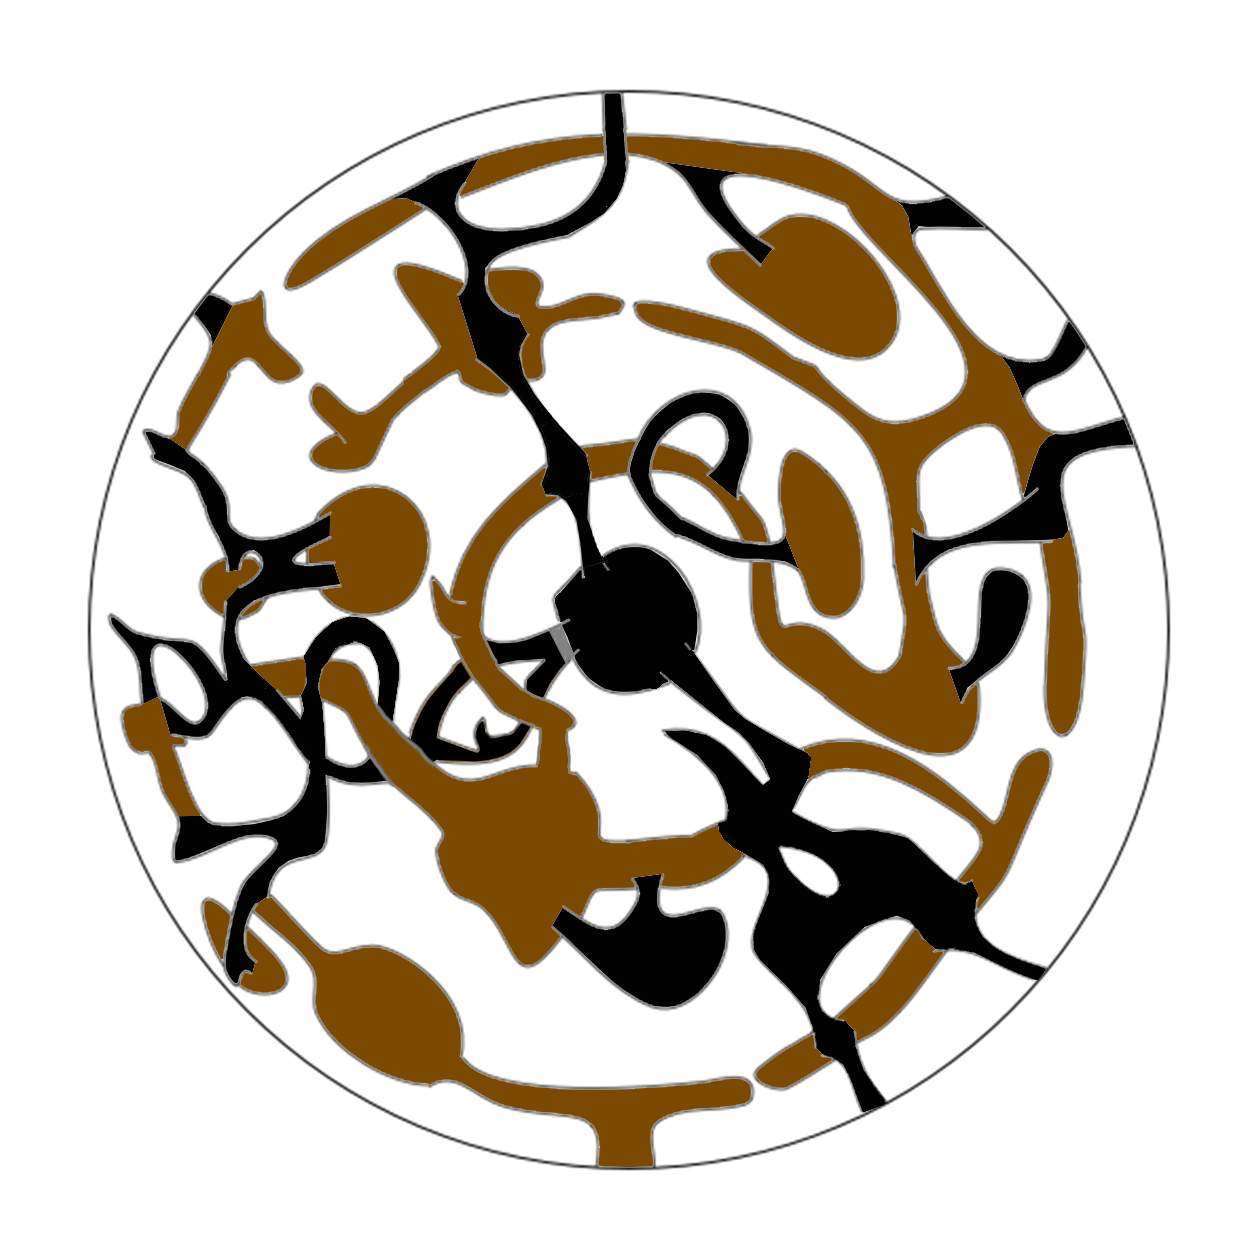
\includegraphics[width=0.6\linewidth]{images/map/2D_map_color.png}
	\caption*{Color}
\end{figure}

\begin{figure}[H]
	\centering
	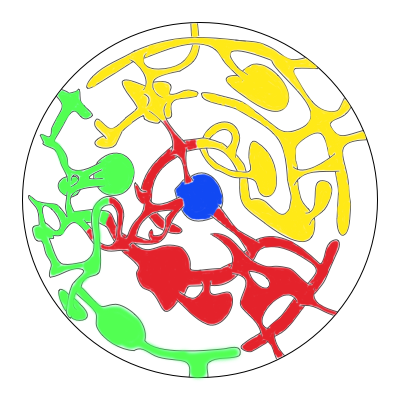
\includegraphics[width=0.6\linewidth]{images/map/map_all_sections.png}
	\caption*{Section 1: green, Section 2: yellow, Section 3: red, Boss Room: blue}
\end{figure}

\begin{figure}[H]
	\centering
	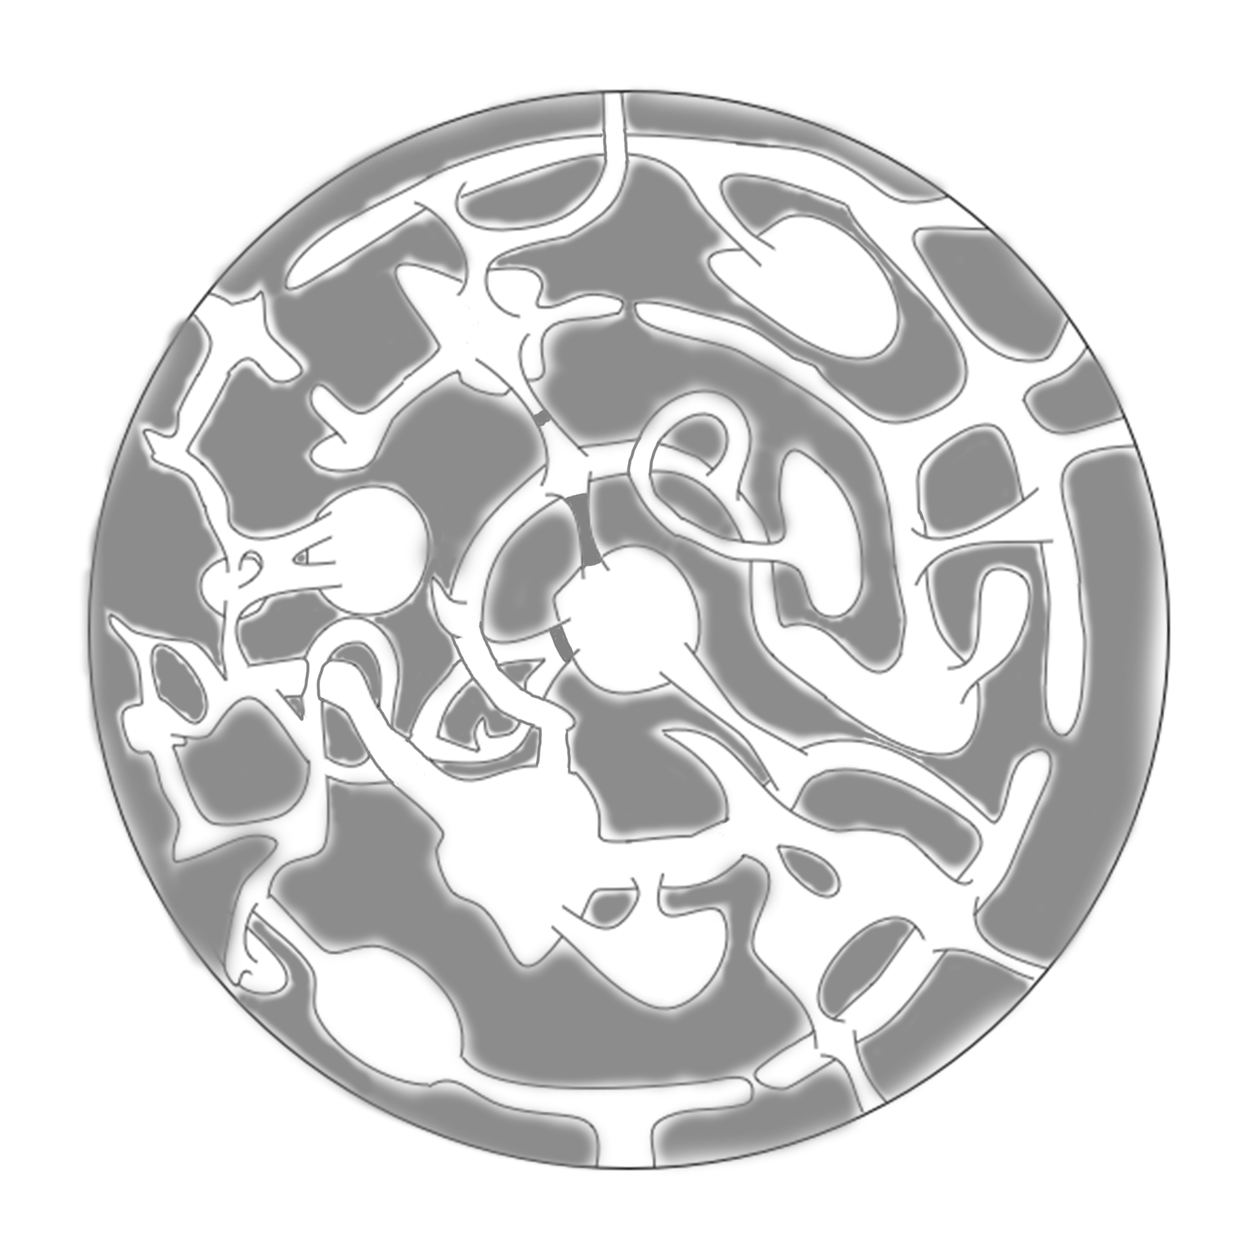
\includegraphics[width=0.6\linewidth]{images/map/2D_map_not.png}
	\caption*{Gray areas cannot be walked on by the player}
\end{figure}
\newpage

\subsubsection{Measures}
\begin{figure}[H]
	\centering
	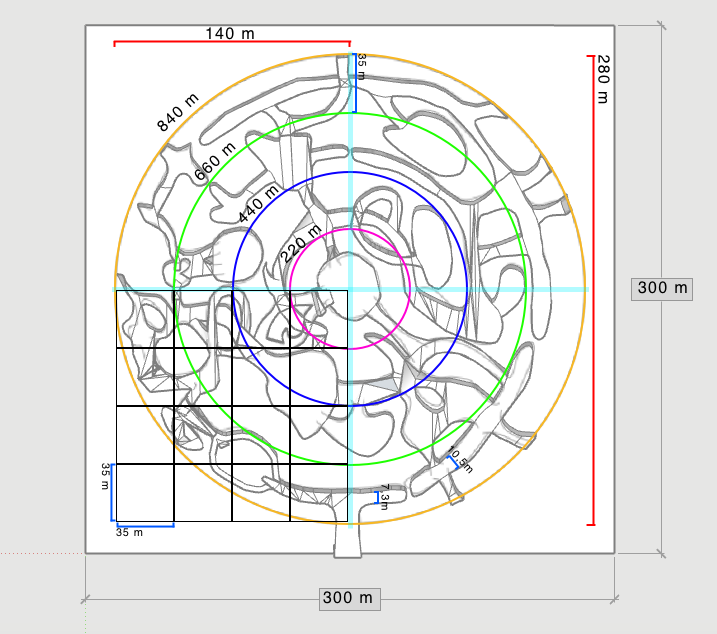
\includegraphics[width=14cm]{images/map/map_measures.png}
\end{figure}

\begin{figure}[H]
	\centering
	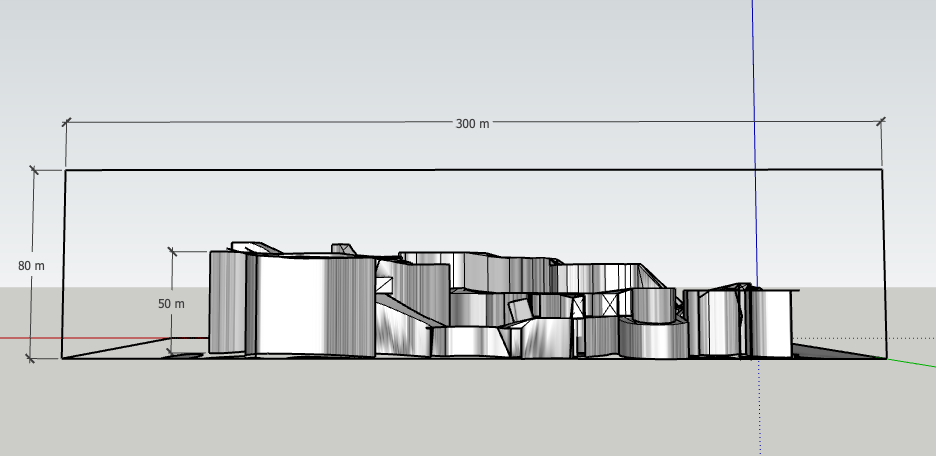
\includegraphics[width=14cm]{images/map/3D_map_half.png}
\end{figure}
\newpage

\subsection{Level Diagram}
\begin{figure}[H]
	\centering
	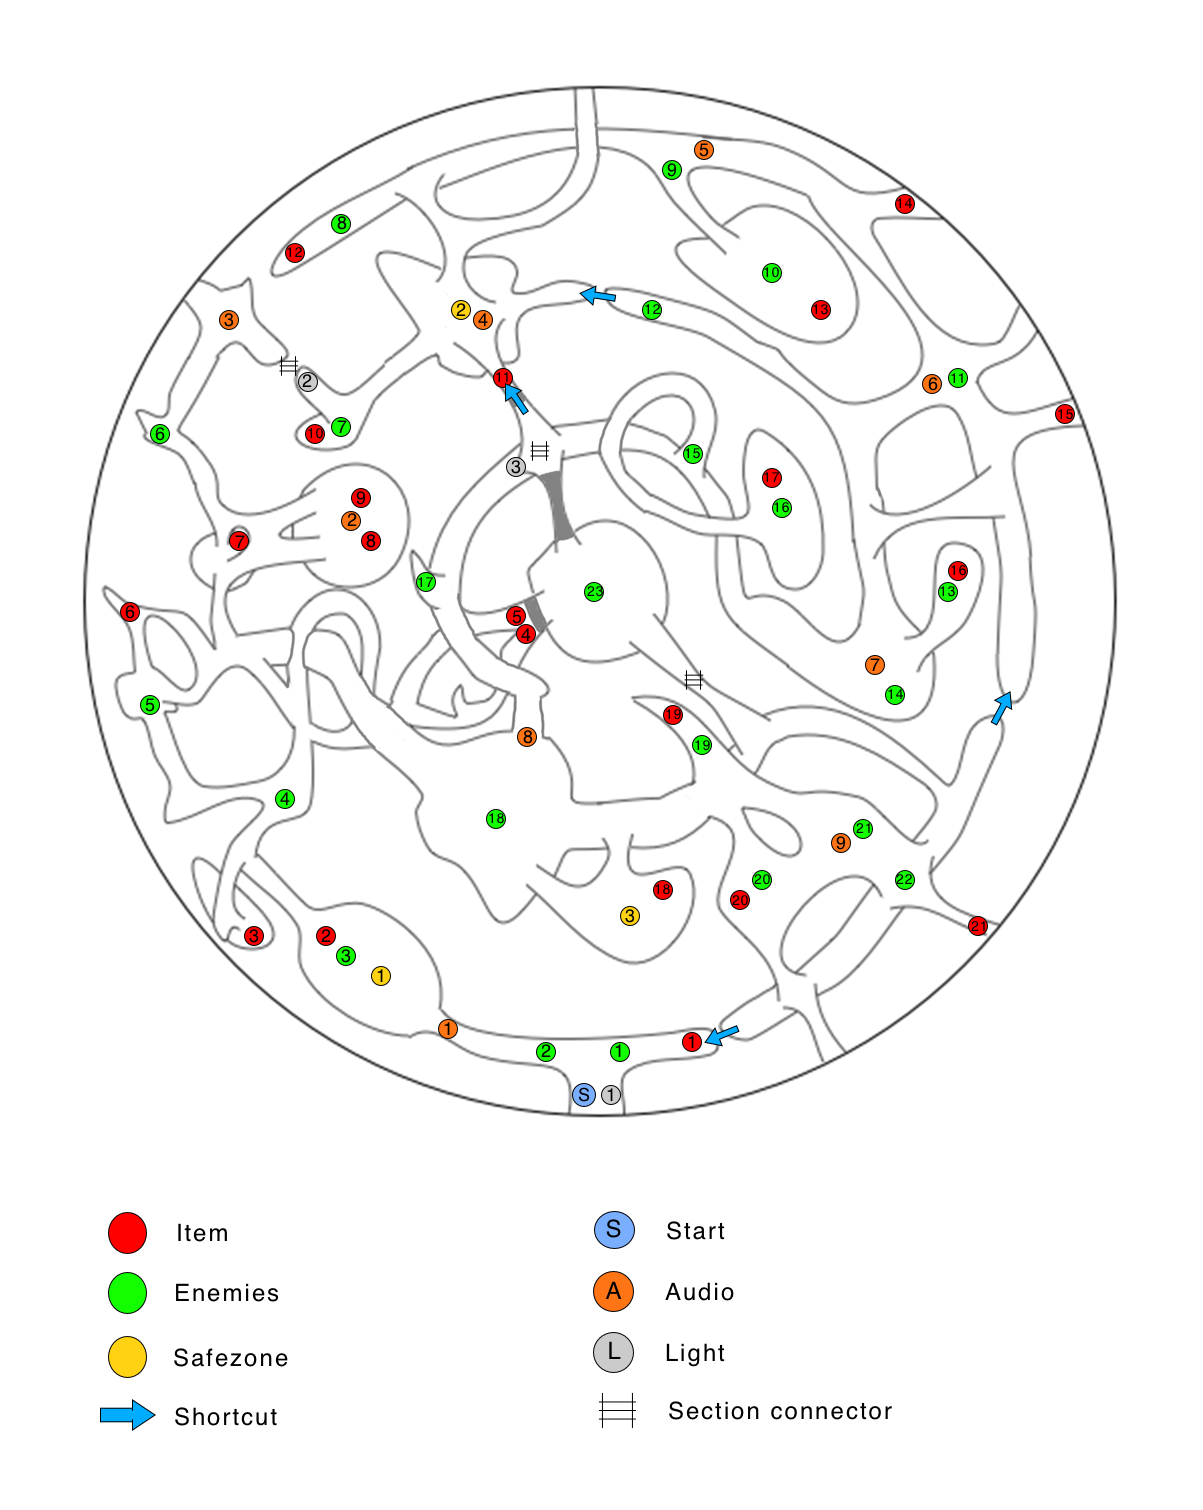
\includegraphics[width=0.95\linewidth]{images/map/map_legend.png}
\end{figure}
\newpage

\subsection{Level Description}
\begin{figure}[H]
	\centering
	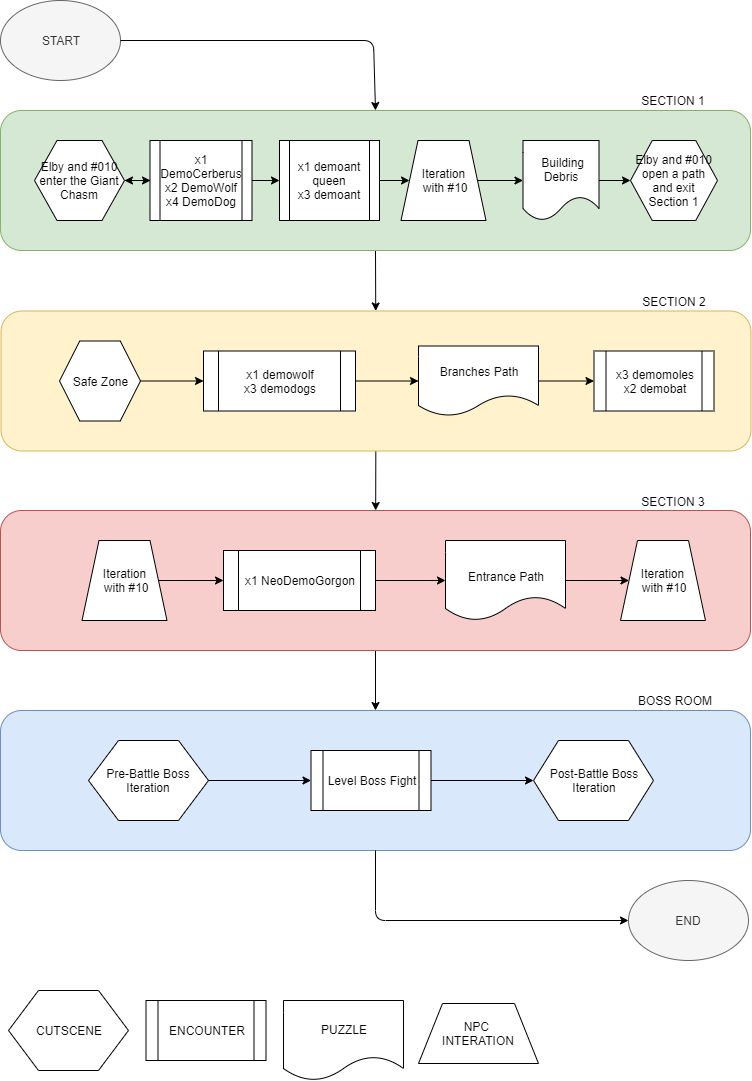
\includegraphics[width=0.95\linewidth]{images/graphs/level_description.png}
\end{figure}
\newpage


\subsubsection{Giant Chasm - Outside}
The level designed is the subarea 15 of the Core Enviroment. It is located in the north side of the City Ruins. The diameter of the giant chasm is at least 300m and its origins are unknown, even if in-game characters often assume that it originated from the impact of a meteorite. From the outside it is impossible to see the contents of the chasm due to the lack of internal light and for the thick crop of vines that surround the entire area. Fixed enemies are placed inside the rooms, while some monsters can randomly spawn along the way.

\begin{figure}[H]
	\centering
	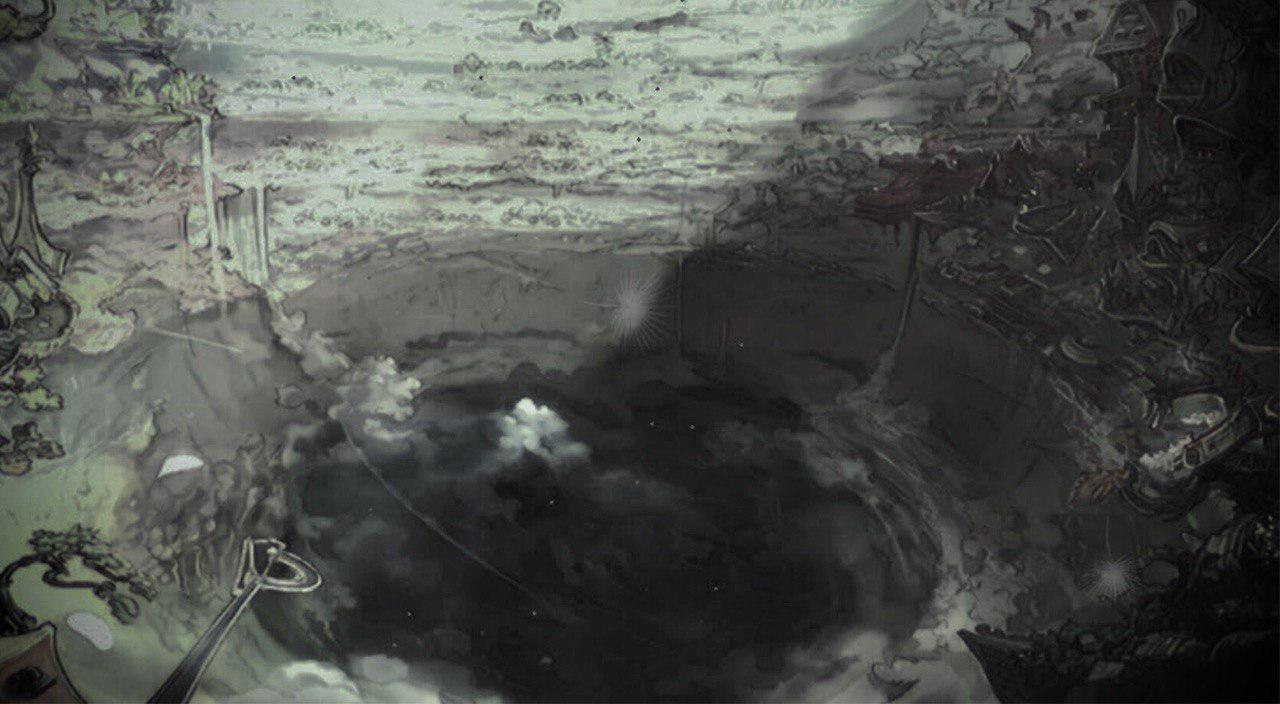
\includegraphics[width=0.8\linewidth]{images/visual_ref/15_giant_chasm/chasm_outside.jpg}
	\caption*{Overview of the Giant Chasm. \textit{[Made in the Abyss]}}
\end{figure}
\newpage


\subsubsection{Giant Chasm - Section 1}
The first section is approximately 500m long and with a variable width depending on the type of terrain (land, vines, etc.). Players enter through a gap in the south side of the Giant Chasm. The left side of the path is blocked by vines and debris and players can only unlock it from the other side in Section 3. Proceeding to the right, players reach the ballroom, where the DemoCerberus stands guard. After the first ruin, players will be forced to continue on the big vines coming from the lower levels of the Chasm, until they returns to the ridge. At the point of descent for the Second Section, it will be necessary to explore the surroundings in order to find a way to break through the obstacle.

\vspace*{0.3cm}
\begin{figure}[H]
	\centering
	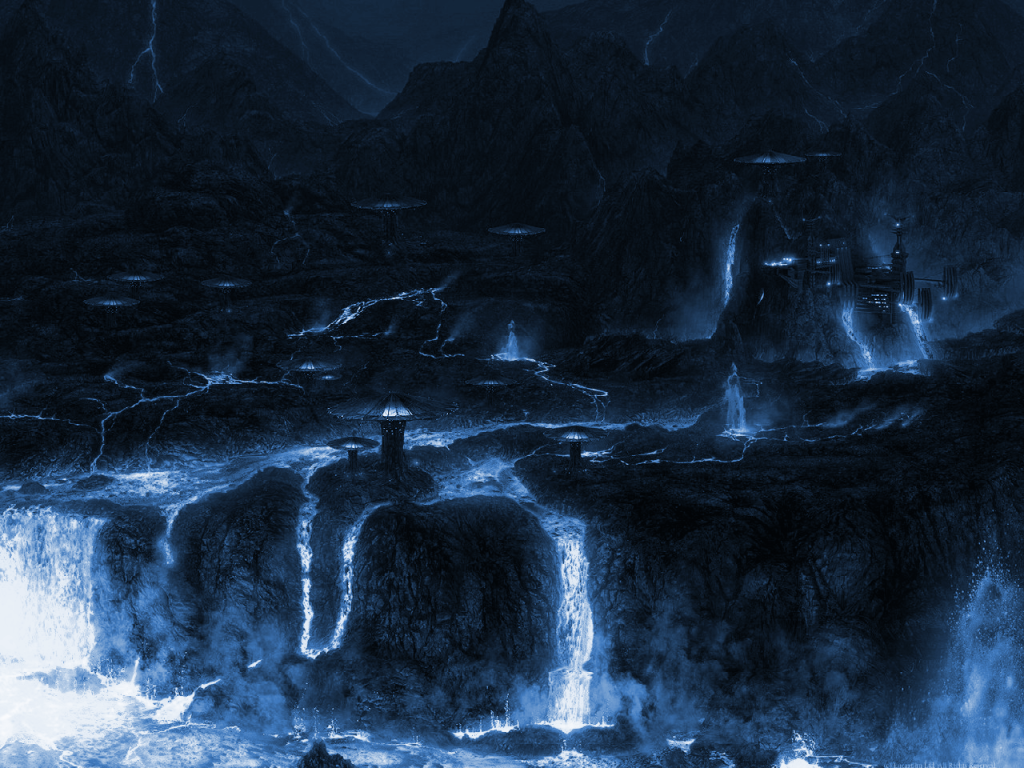
\includegraphics[width=0.7\linewidth]{images/visual_ref/15_giant_chasm/chasm_section_1.png}
	\caption*{Path of the first section}
\end{figure}

\begin{figure}[H]
	\centering
	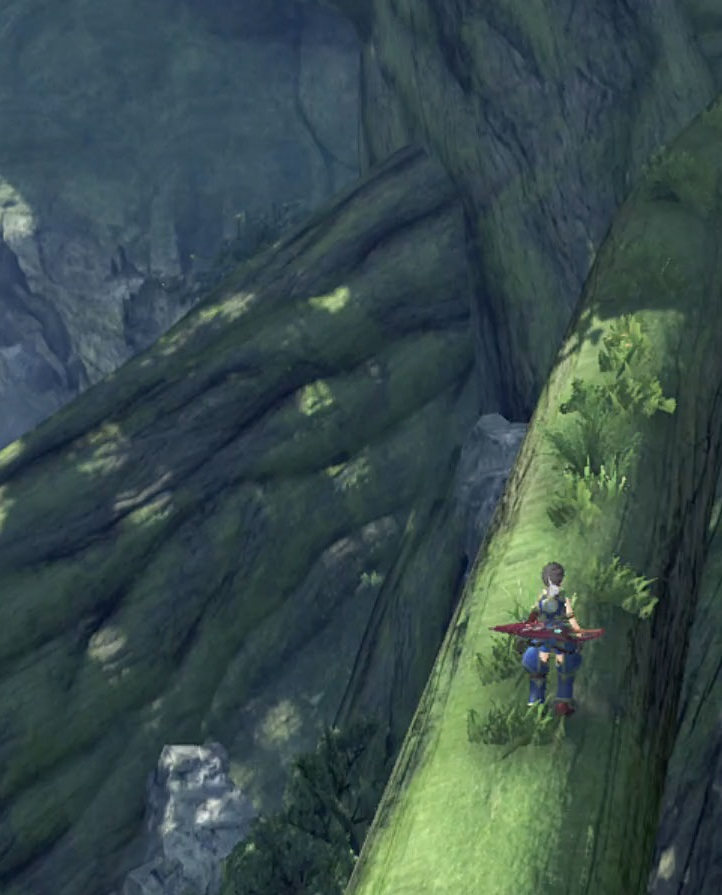
\includegraphics[width=0.5\linewidth]{images/visual_ref/15_giant_chasm/tree.jpg}
\end{figure}

\begin{figure}[H]
	\centering
	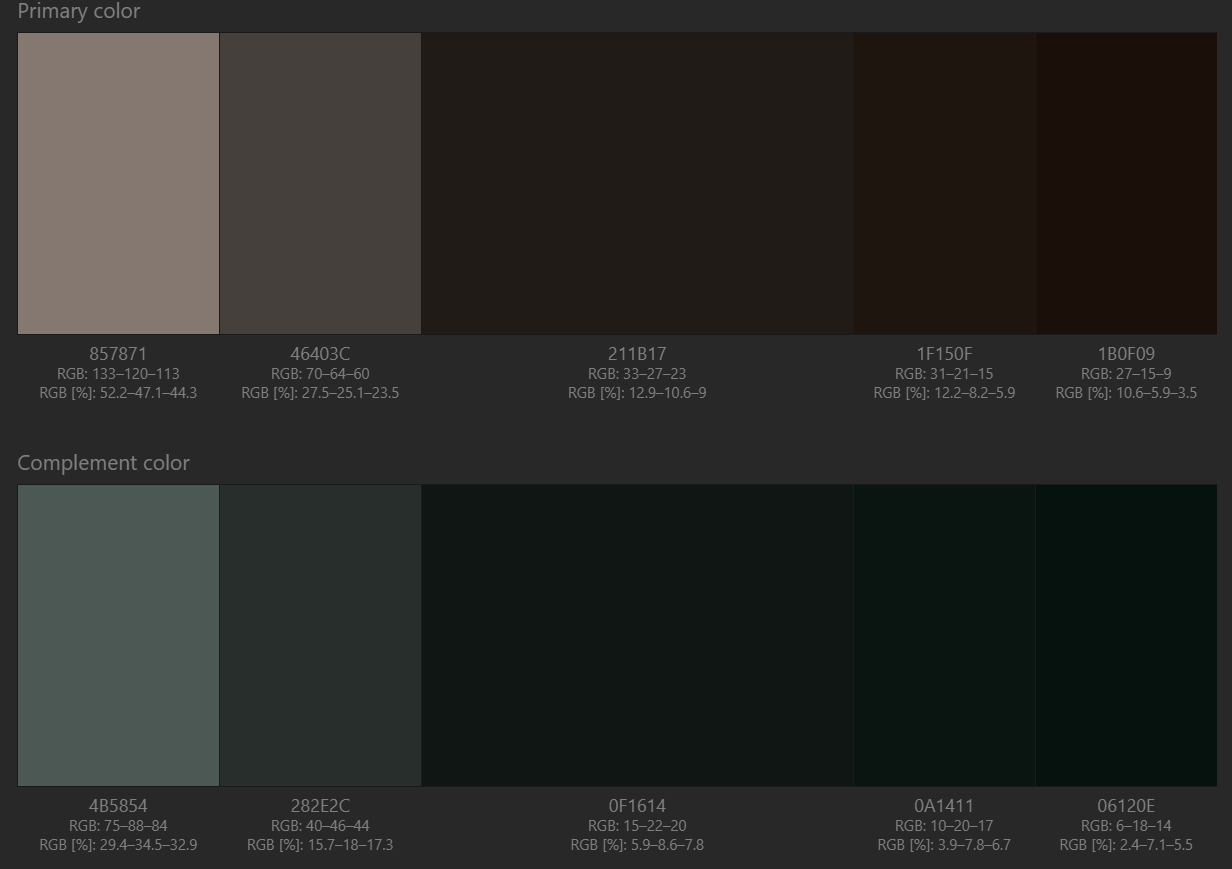
\includegraphics[width=0.8\linewidth]{images/visual_ref/15_giant_chasm/pallette/pallette_section_01.png}
\end{figure}

\begin{figure}[H]
	\centering
	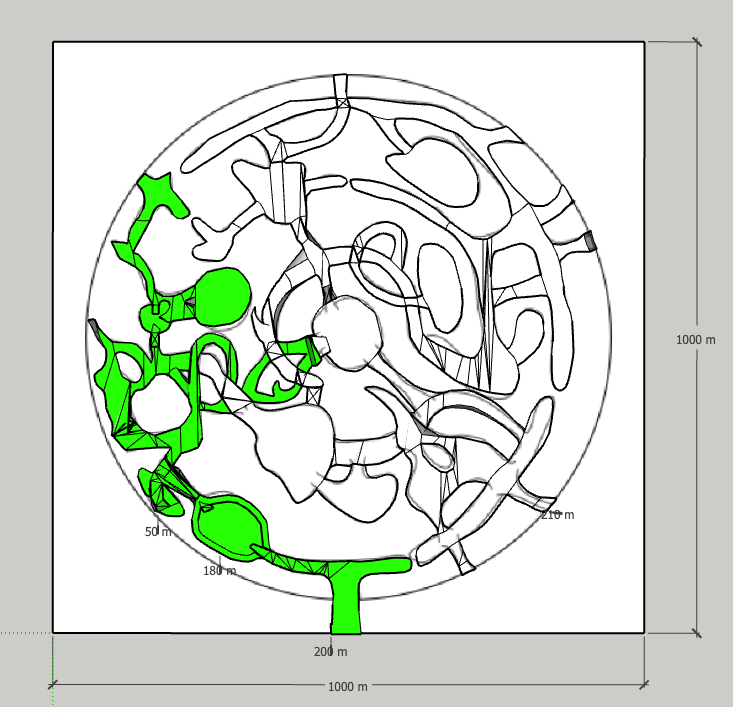
\includegraphics[width=0.7\linewidth]{images/map/2D_map_section_01.png}
	\caption*{Section 1}
\end{figure}

\begin{figure}[H]
	\centering
	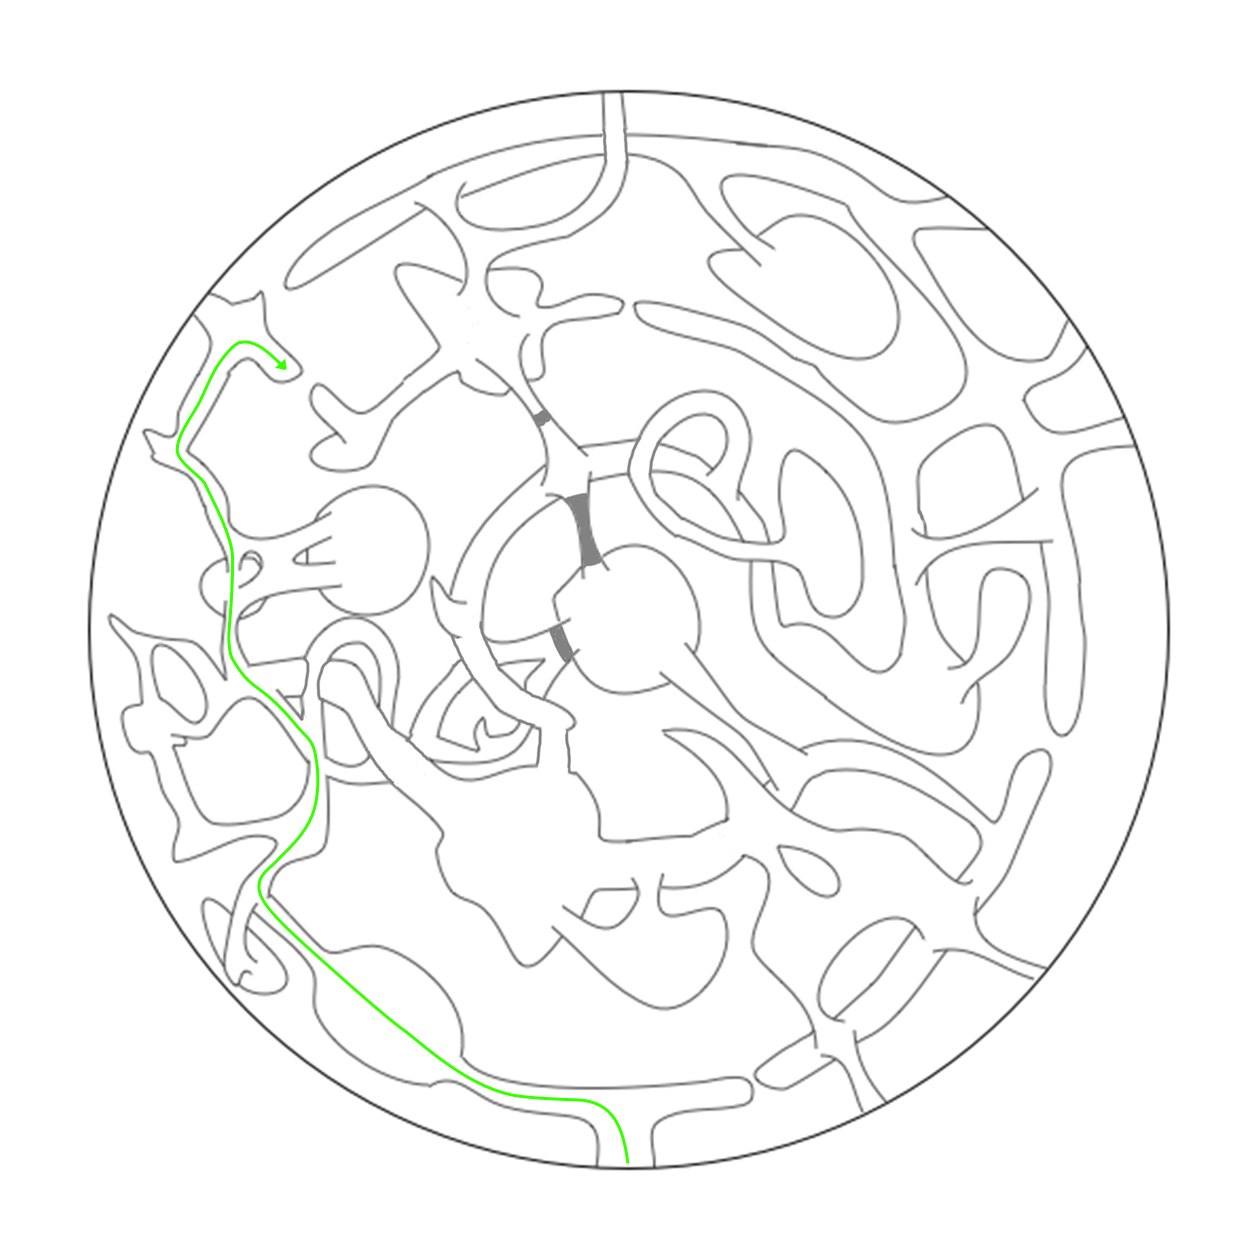
\includegraphics[width=0.7\linewidth]{images/map/map_principle_path_section_01.png}
	\caption*{Section 1 main path}
\end{figure}


\textbf{Encounters}
\begin{itemize}
	\item 1x DemoCerberus
	\item 2x DemoWolf
	\item 4x DemoDog
\end{itemize}
The Democerberus is considered a mini-boss and its statistics are proportionally reduced compared to its previous Level Boss version. At the entrance to the room, the DemoCerberus, previously in a resting position, enters an offensive state, remaining however to guard the exit of the ruin. Once the first damage threshold has been exceeded, the monster will recall two DemoWolves, which will immediately attack the players. Until the DemoWolves are defeated, the DemoCerberus will not attack and will be invulnerable. Ultimatly, upon reaching the second threshold, the Democerberus will call up four DemoDogs and it will apply the previous pattern.

\begin{itemize}
	\item 1 - 50\% Demorat, 30\% Demobat, 20\% Demodog
	\item 2 - 15\% Demowolves, 35\% Demobat, 50\% Demodog
	\item 3 - Democerberus x1
	\item 4 - 50\% Demorat, 30\% Demobat, 20\% Demodog
	\item 5 - 50\% Demorat, 30\% Demobat, 20\% Demomoles
	\item 6 - 20\% Demomoles, 60\% Demobat, 20\% Demodog
\end{itemize}

\newpage

\textbf{Sounds}\\
DemoDog / DemoWolf howls can be heard randomly. Near the ruins there is a sound of landslides. The sound of Elby's footsteps changes according to the terrain on which she is located.

\begin{itemize}
	\item 1 - Howling wolves
	\item 2 - Moaning monsters
	\item 3 - Landslide noise
\end{itemize}

\textbf{Lighting}\\
There's a soft white light coming from the few opening in the crop of vines. It is also possible to see a slight red light coming from the chasm center. The rooms in the ruins are illuminated by a strange luminous moss.

\begin{itemize}
	\item 1 - Trigger light change
\end{itemize}

\textbf{Drops}
\begin{itemize}
	\item 1 - Fresh moss
	\item 2 - Rooten potion
	\item 3 - Rotten root
	\item 4 - Demowolf Tooth
	\item 5 - Fresh root
	\item 6 - Rotten moss
	\item 7 - Rotten moss
	\item 8 - Fresh elisir
	\item 9 - Demorat Tail
\end{itemize}

\textbf{Puzzle}\\
To change area Elby will find herself facing a bridge of dry and weak vines. At this point, in order to be able to move on, she will need to freeze the vines so as to strengthen them.\\
The path melts very quickly so that the protagonist can only cross each box once. once all the quadrants are weakened, the block will break making it fall. Elby will therefore have to be at the point indicated by the X in the image below in order to continue his journey. If this does not happen, \#010 will repeat the reconstruction of the bridge to prevent it from falling and injuring Elby. The latter will lose a quarter of its life and will have to repeat the operation.\\
The path can be solved as follows:\\

\newpage

\textit{Main Solution}\\
up / left x2 / up x4 / right / down x3 / right x2 / down / right / up x4 / left / down x2 / left / up x2\\

\begin{figure}[H]
	\centering
	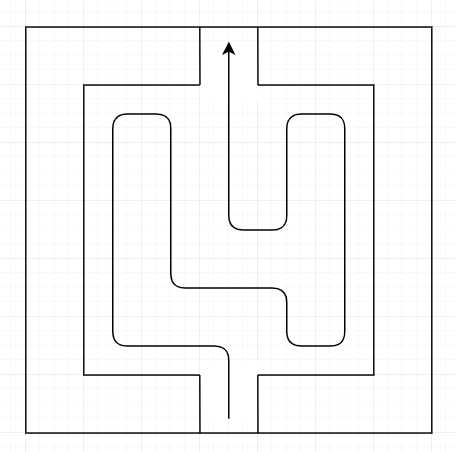
\includegraphics[width=0.5\linewidth]{images/puzzle/puzzle_011.png}
\end{figure}

\textit{Alternative Solution}\\
up / left x2 / up x2 / right / down / right x2 / down / right / up x4 / left / down x2 / left / up / left x2 / up / right x2 / up\\

\begin{figure}[H]
	\centering
	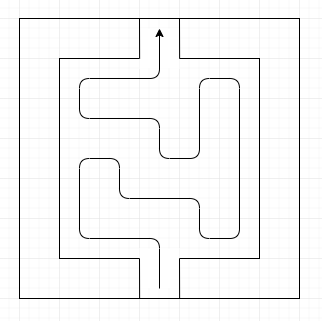
\includegraphics[width=0.5\linewidth]{images/puzzle/puzzle_012.png}
\end{figure}
\newpage


\subsubsection{Giant Chasm - Section 2}
The second section is about 4 km long and takes players to the first underground layer.
Compared to Section 1, the route is narrower and made up of tunnels that allow you to move upwards or downwards and reach platforms and / or ridges that cannot be accessed in other ways. Players will often be asked to use skills to open passages and / or move debris. The soil, where it is not covered with organic vines, is very irregular due to the proximity of the nucleus and the presence of many DemoMoles. Players will find a Safe Room near the beginning of Section 2, and they will unlock a path to reach the room again just before Section 3.

\vspace*{0.3cm}
\begin{figure}[H]
	\centering
	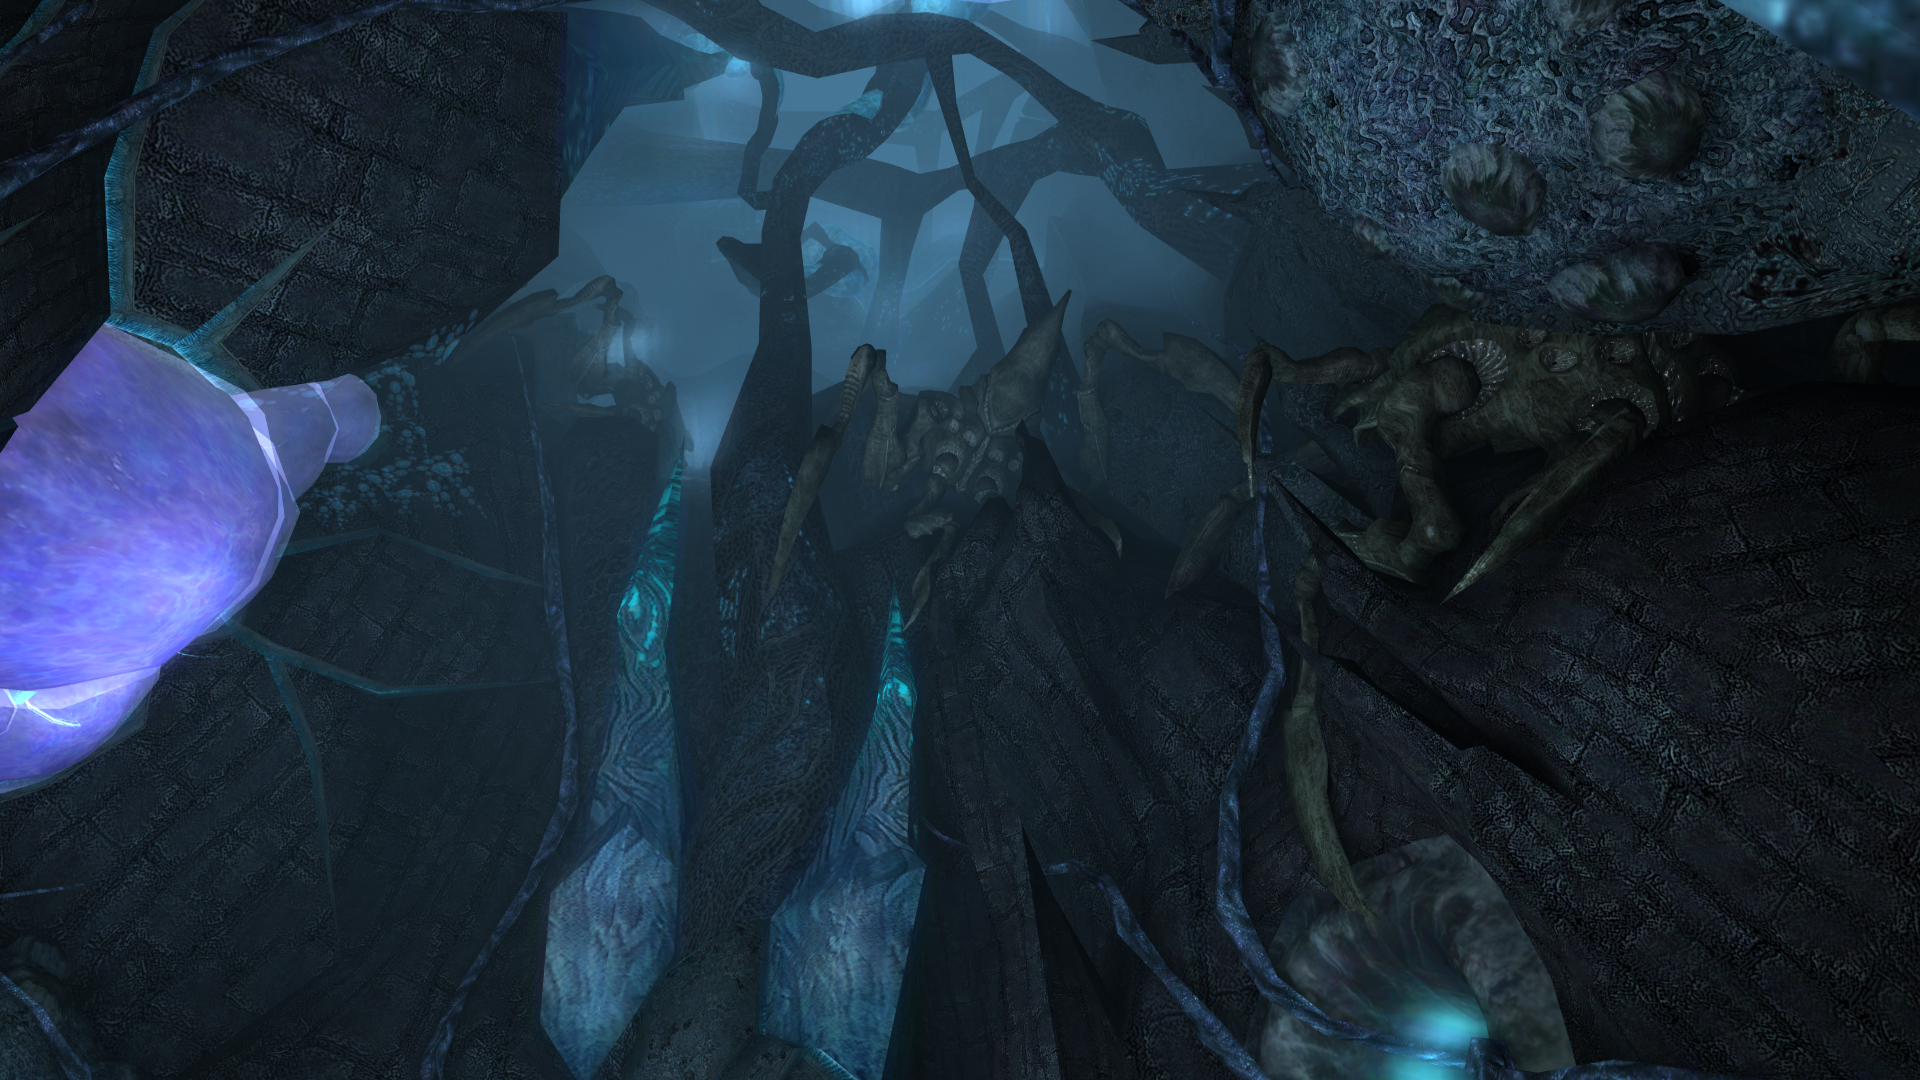
\includegraphics[width=0.8\linewidth]{images/visual_ref/15_giant_chasm/chasm_section_2.png}
	\caption*{Path of the second section}
\end{figure}

\begin{figure}[H]
	\centering
	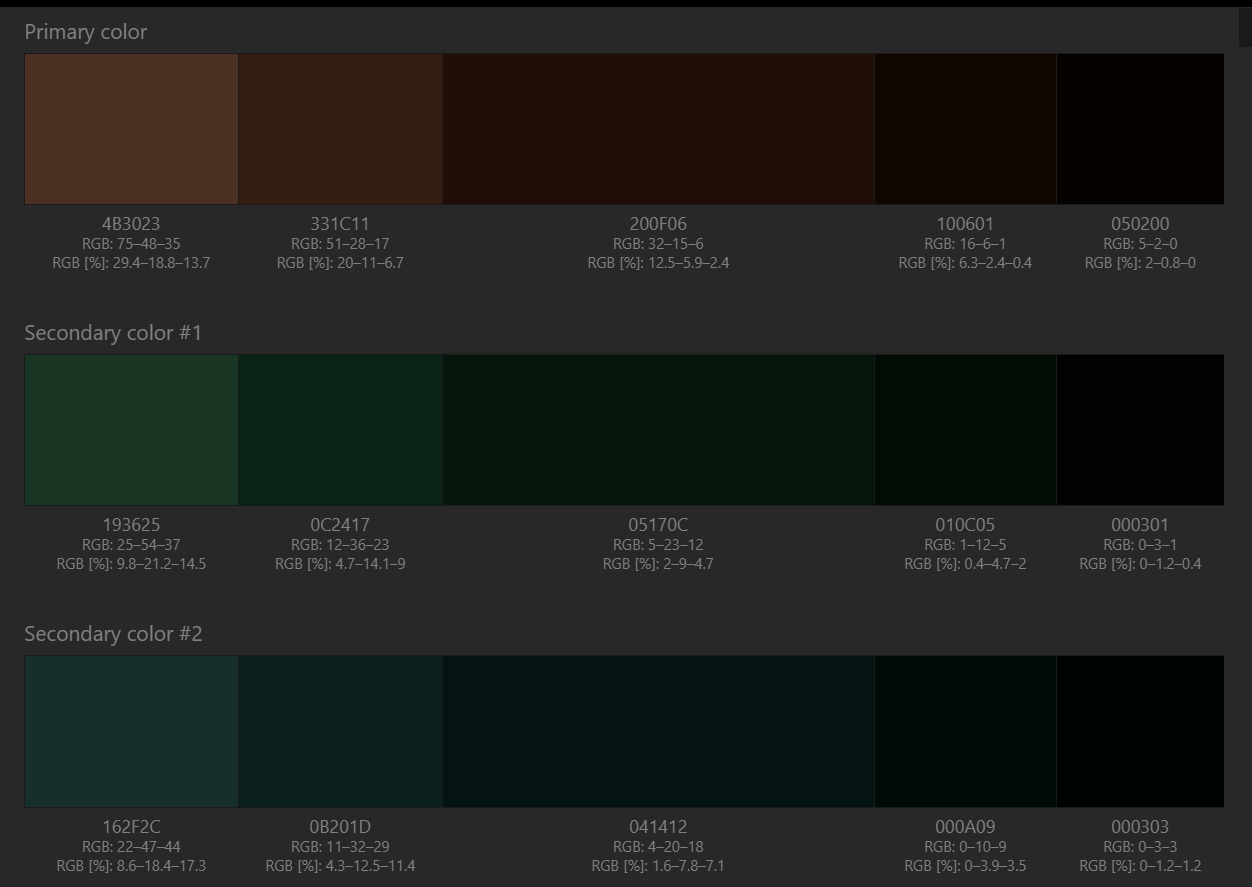
\includegraphics[width=0.8\linewidth]{images/visual_ref/15_giant_chasm/pallette/pallette_section_02.png}
\end{figure}

\begin{figure}[H]
	\centering
	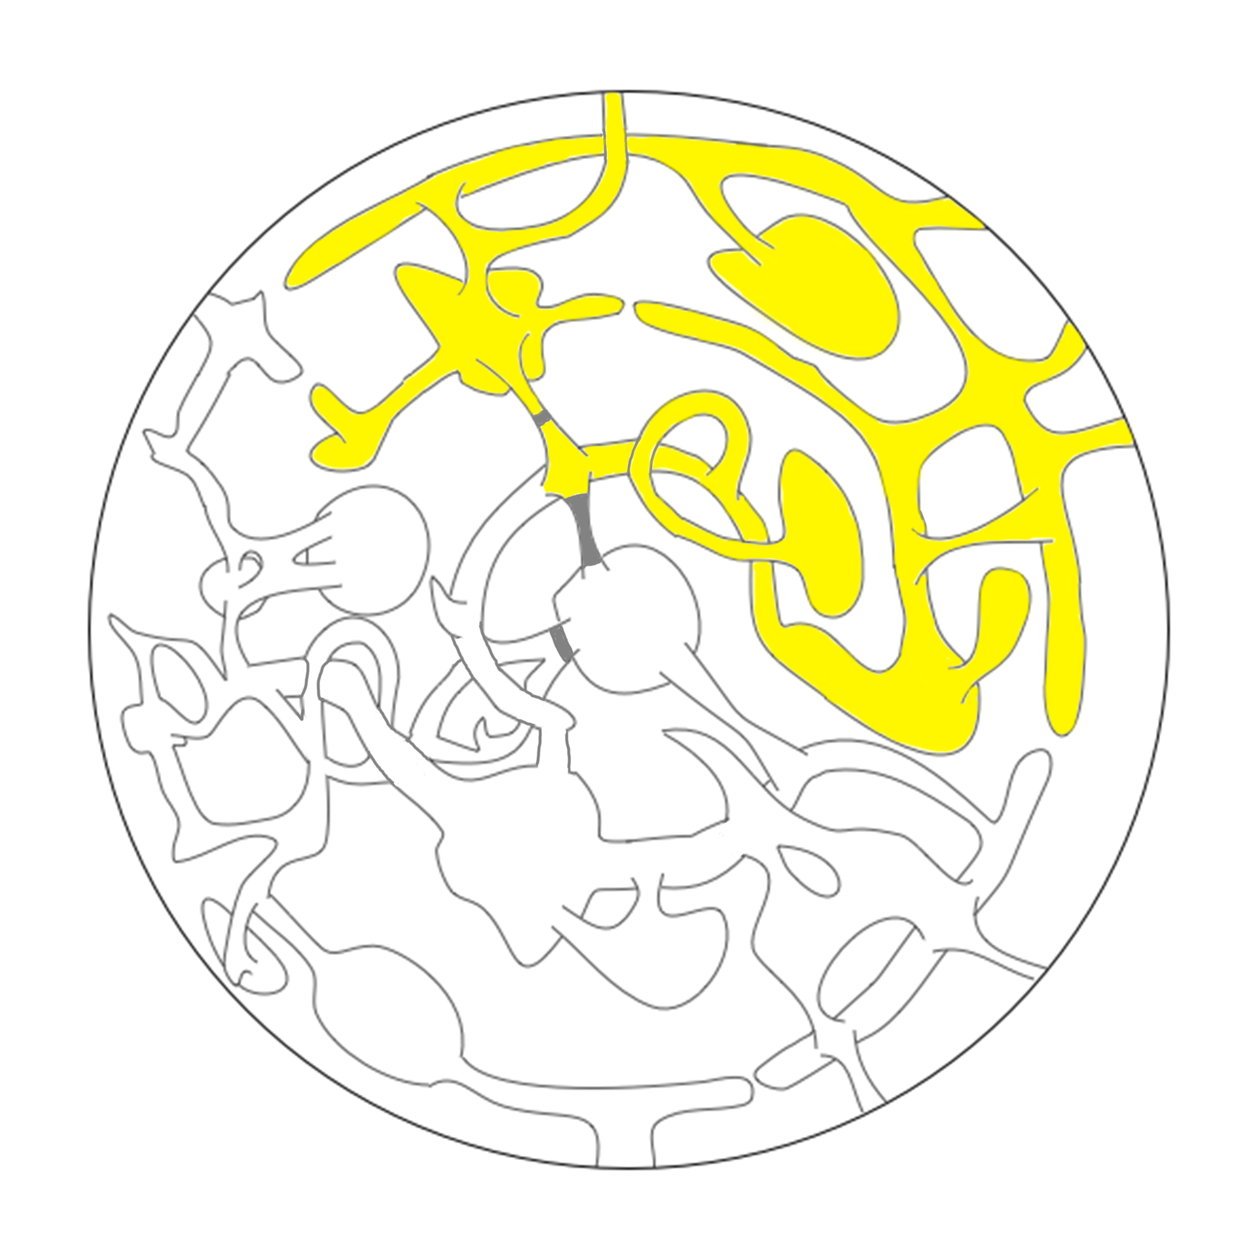
\includegraphics[width=0.7\linewidth]{images/map/2D_map_section_02.png}
	\caption*{Section 2}
\end{figure}

\begin{figure}[H]
	\centering
	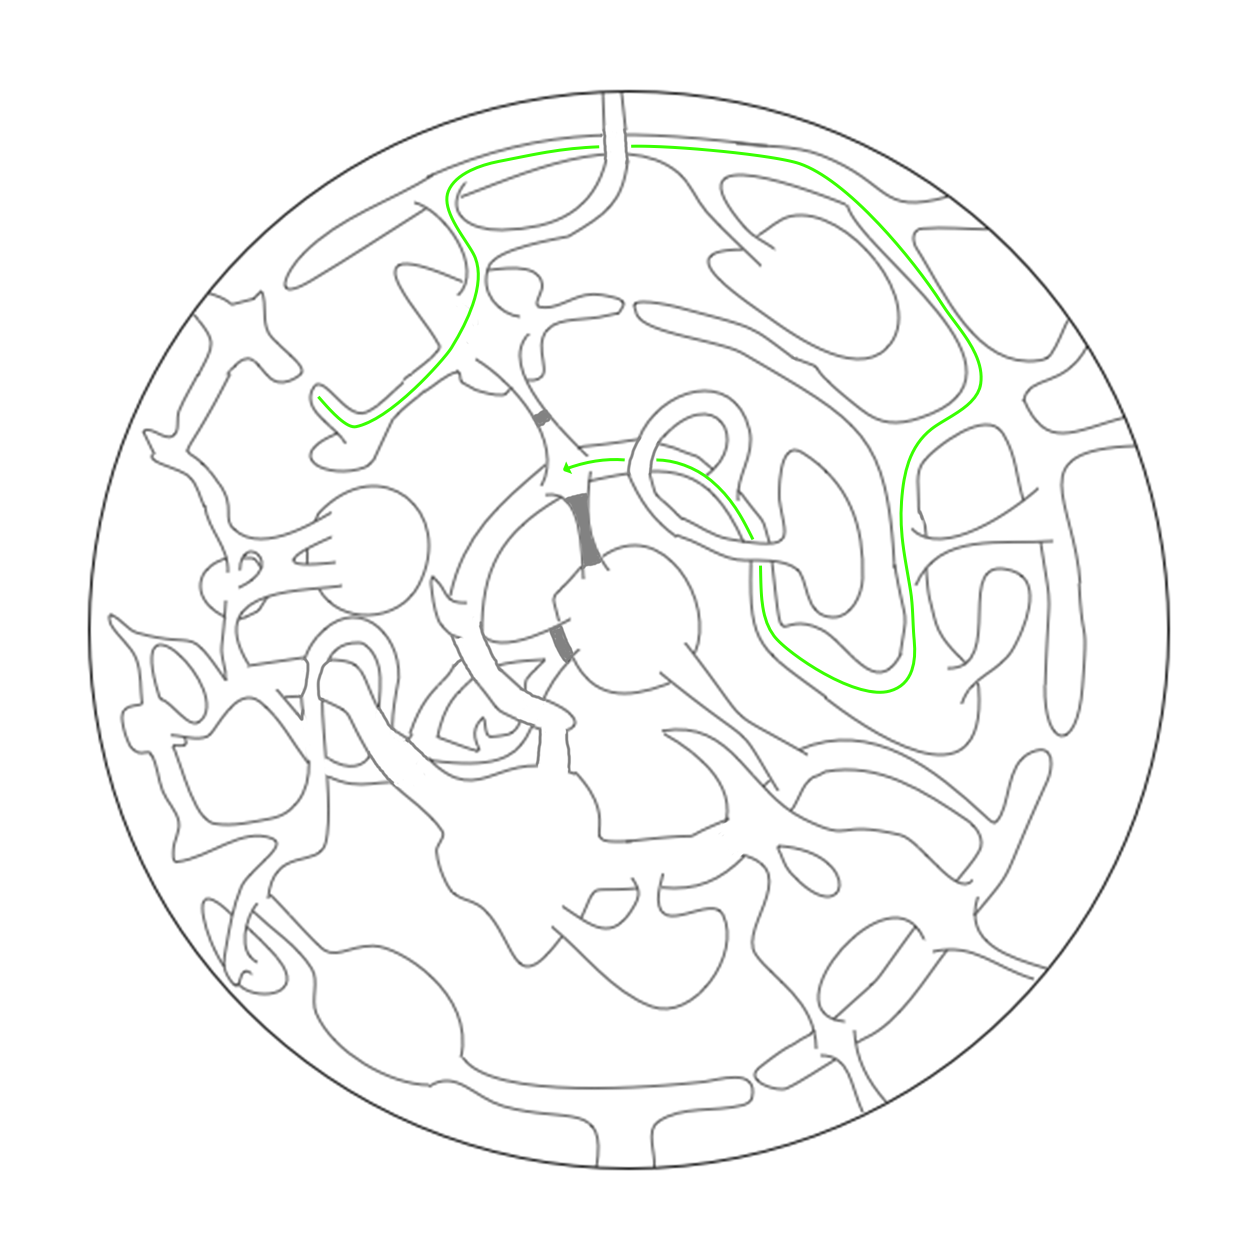
\includegraphics[width=0.7\linewidth]{images/map/map_principle_path_section_02.png}
	\caption*{Section 2 main path}
\end{figure}

\textbf{Encounter A}
\begin{itemize}
	\item x1 DemoWolf
	\item x2 DemoDog
\end{itemize}
A herd of DemoWolf. Players can kill DemoDogs one at a time to deal individually with the DemoWolf. Otherwise, if the DemoWolf is alerted, it will trigger all the DemoDogs in the room.\\

\textbf{Encounter B}
\begin{itemize}
	\item x2 DemoMoles
	\item x1 DemoBat
\end{itemize}
Entering the ruin, the player will find it empty. Once in the middle of the room, Elby and \#010 will remain stuck in the ground, and the player will have a few seconds to activate the Levitation skill to avoid taking damage (Quick Time Event). Finally, the DemoMoles and DemoBats will appear, starting the battle.

\begin{itemize}
	\item 7 - 50\% Demorat, 30\% Demobat, 20\% Demodog
	\item 8 - 20\% Demorat, 60\% Demobat, 20\% Demodog
	\item 9 - 15\% Demowolves, 35\% Demobat, 50\% Demodog
	\item 10 - 50\% Demorat, 30\% Demobat, 20\% Demodog
	\item 11 - 20\% Demobat, 60\% Demorat, 20\% Demodog
	\item 12 - 50\% Demorat, 30\% Demobat, 20\% Demodog
	\item 13 - Demowolf x1, Demodog x2
	\item 14 - 20\% Demorat, 60\% Demobat, 20\% Demodog
	\item 15 - 40\% Demorat, 40\% Demobat, 20\% Demomoles
	\item 16 - Demomoles x2, Demobat x1
\end{itemize}


\textbf{Sounds}\\
The rustling of moving vines can be heard randomly. The sound of Elby's footsteps changes according to the terrain on which she is located.

\begin{itemize}
	\item 4 - Landslide
	\item 5 - Flapping of wings
	\item 6 - Whoosh vines
	\item 7 - Landslide
\end{itemize}

\textbf{Lighting}\\
There's no light coming from above. The only lights are the white one coming from the moss and the red one coming from the core (more intense than Section 1).

\begin{itemize}
	\item 2 - Trigger light change
\end{itemize}

\newpage

\textbf{Drops}
\begin{itemize}
	\item 10 - Rotten elisir
	\item 11 - Monster meat
	\item 12 - Demorat Tail
	\item 13 - Fresh root
	\item 14 - Demowolf Tooth
	\item 15 - Rotten root
	\item 16 - Rotten moss
	\item 17 - Demorat Tail
\end{itemize}

\textbf{Puzzle}\\
Bad Eleven will find the street blocked by a lot of rocks. So she has to push them away, in the correct order, with his special mental ability. When there are no more moves available or the puzzle is irreversibly unsolvable, a dialogue line of \#010 will appear and then the room will be reset.
The path can be solved as follows:\\

\begin{figure}[H]
	\centering
	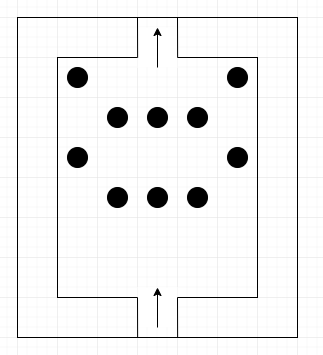
\includegraphics[width=0.7\linewidth]{images/puzzle/puzzle_021.png}
\end{figure}

\begin{figure}[H]
	\centering
	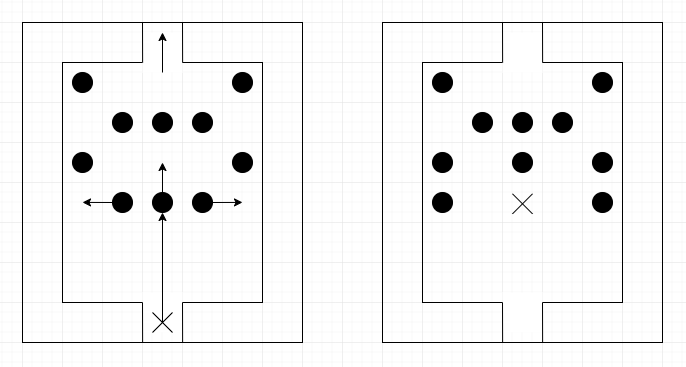
\includegraphics[width=0.8\linewidth]{images/puzzle/puzzle_022.png}
	\caption*{First step}
\end{figure}

\begin{figure}[H]
	\centering
	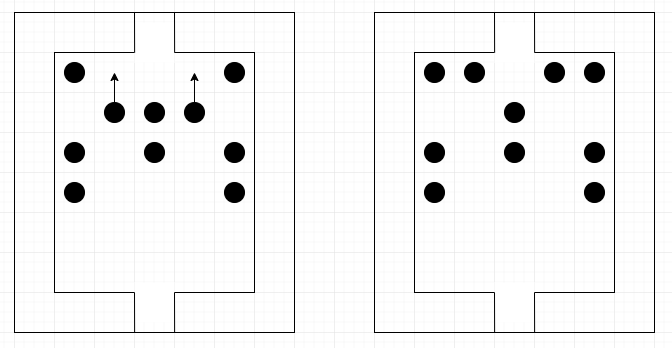
\includegraphics[width=0.8\linewidth]{images/puzzle/puzzle_023.png}
	\caption*{Second step}
\end{figure}

\begin{figure}[H]
	\centering
	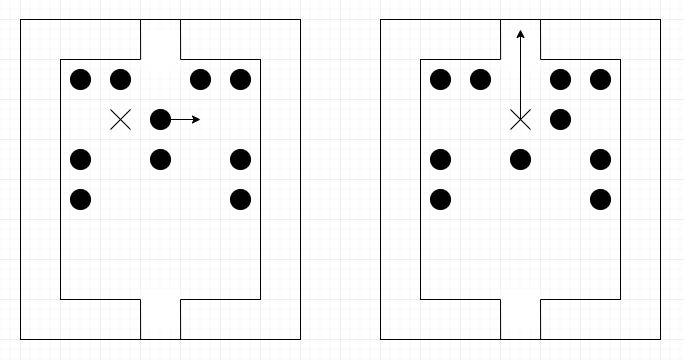
\includegraphics[width=0.8\linewidth]{images/puzzle/puzzle_024.png}
	\caption*{Third step}
\end{figure}
\newpage

\subsubsection{Giant Chasm - Section 3}
The third and final section is about 300m long and brings players to the second underground layer. It is not possible to follow any terrain course, forcing the players to climb and descend from the multitude of organic vines coming from the core, now extremely close. In this section players can explore the ramifications to obtain useful items and / or unlock the passage to the entrance of the abyss, allowing a possible backtracking. Following the main path and after facing the NeoDemoGorgon in his den, the player finally arrives in front of the gap for the heart of the Giant Chasm.

\vspace*{0.3cm}
\begin{figure}[H]
	\centering
	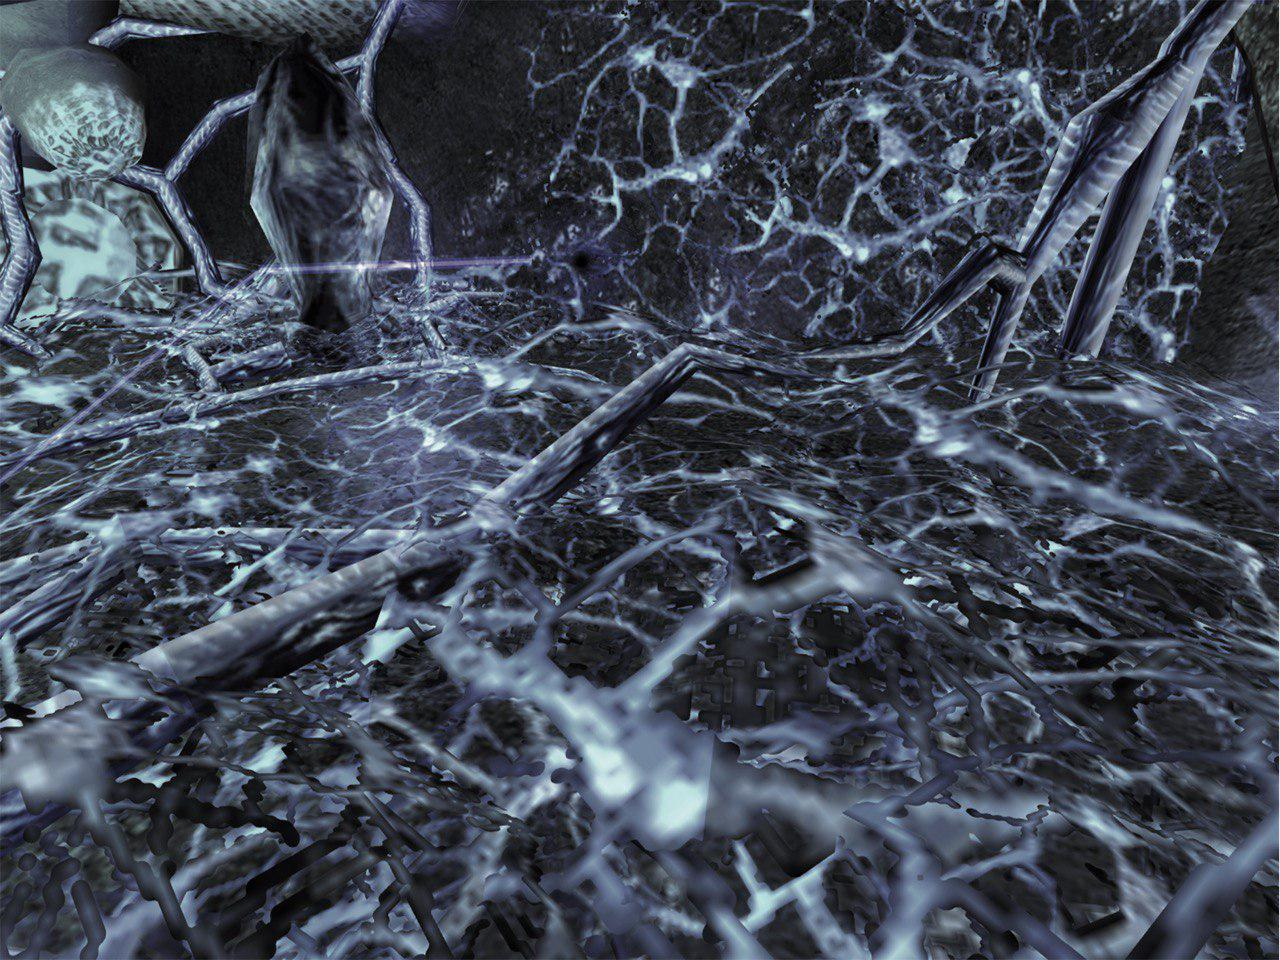
\includegraphics[width=0.8\linewidth]{images/visual_ref/15_giant_chasm/chasm_section_3.jpg}
	\caption*{Ground in the third section}
\end{figure}

\begin{figure}[H]
	\centering
	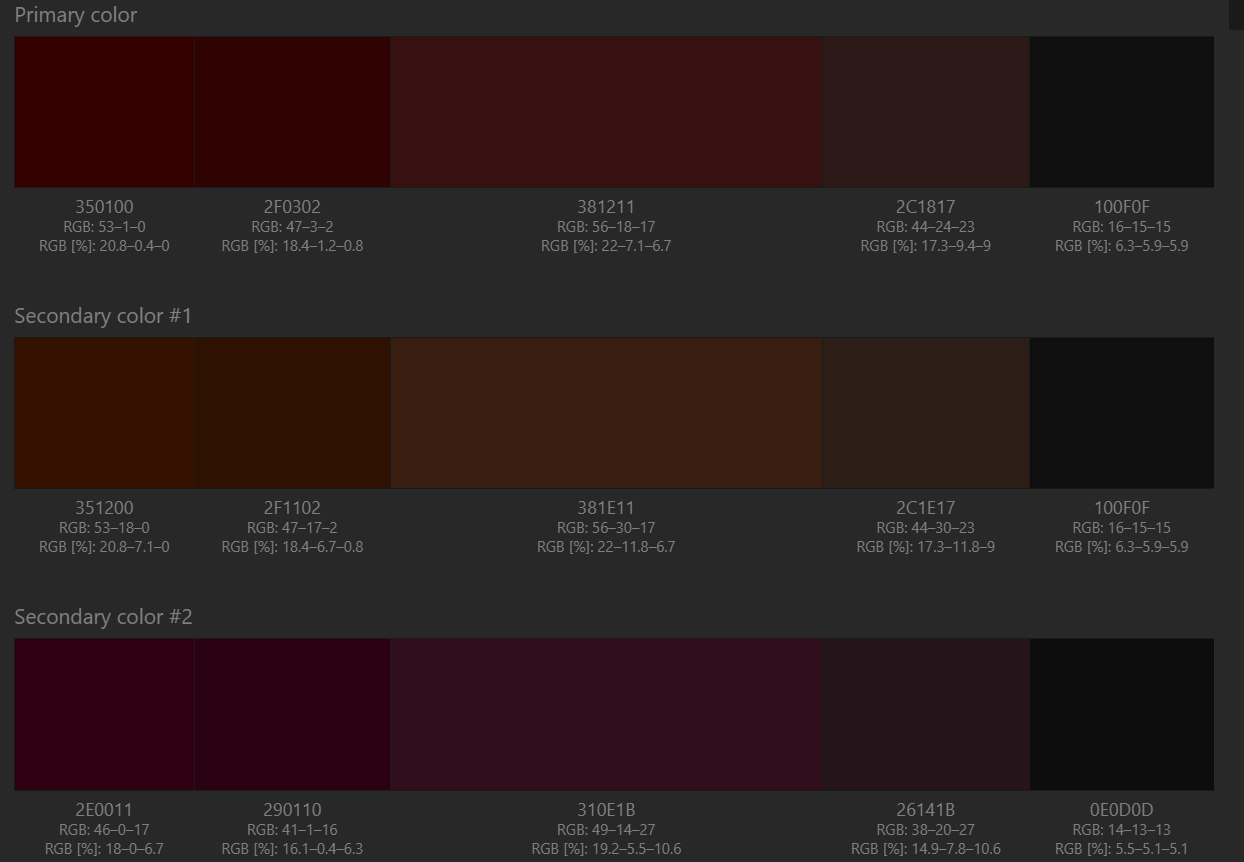
\includegraphics[width=0.8\linewidth]{images/visual_ref/15_giant_chasm/pallette/pallette_section_03.png}
\end{figure}

\begin{figure}[H]
	\centering
	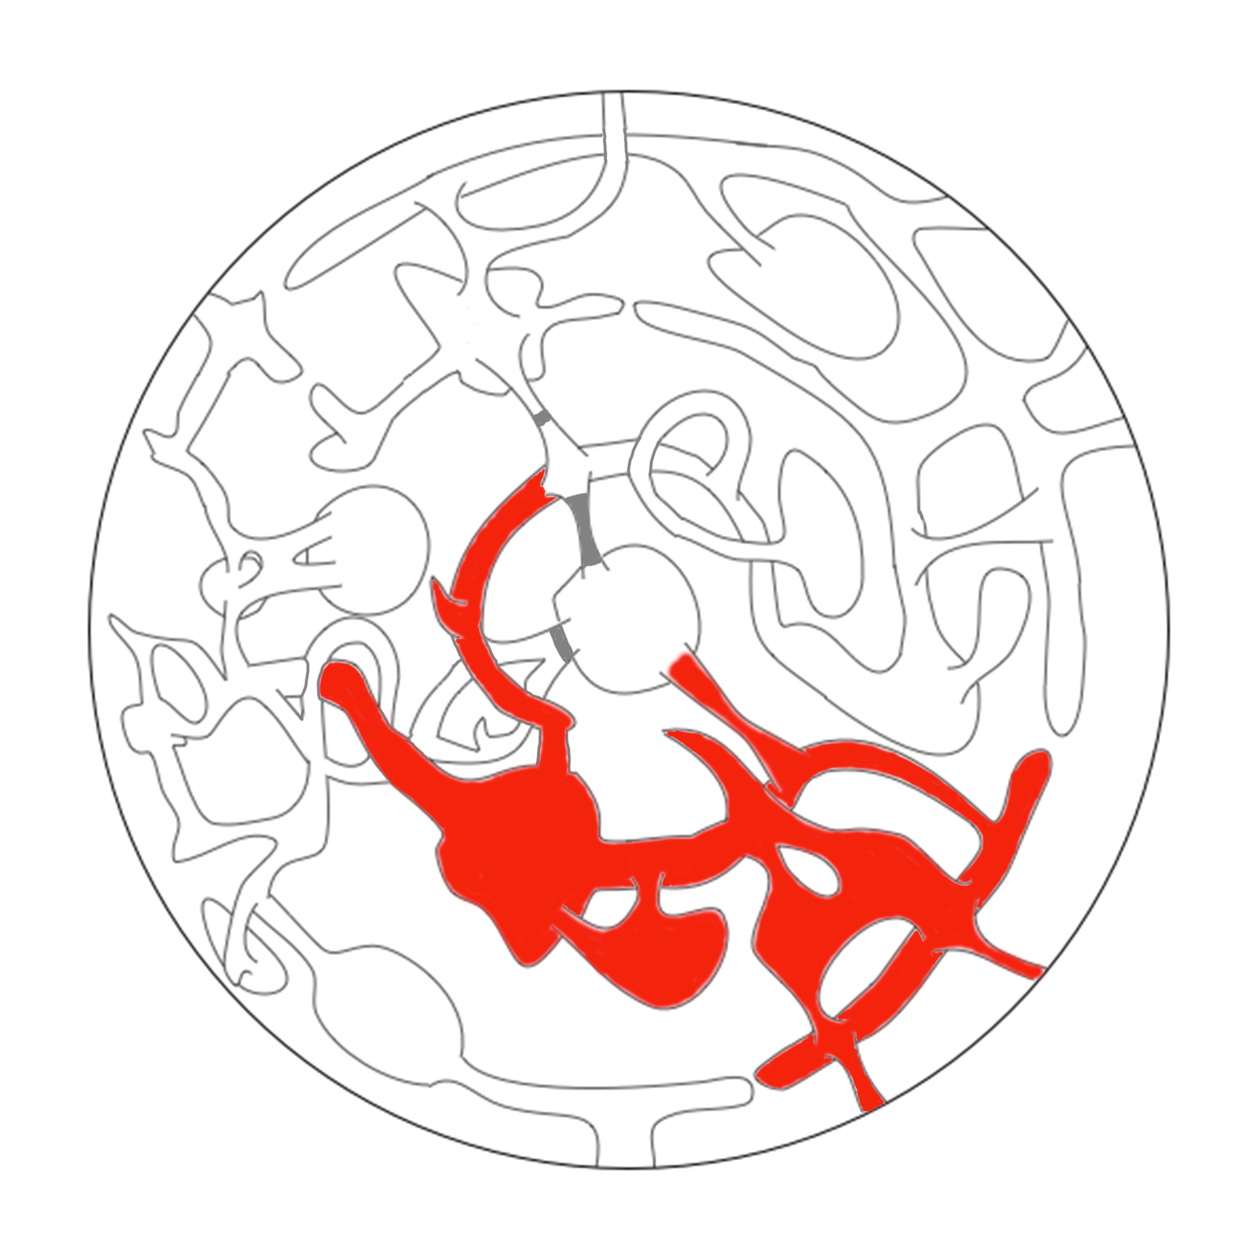
\includegraphics[width=0.7\linewidth]{images/map/2D_map_section_03.png}
	\caption*{Section 3}
\end{figure}

\begin{figure}[H]
	\centering
	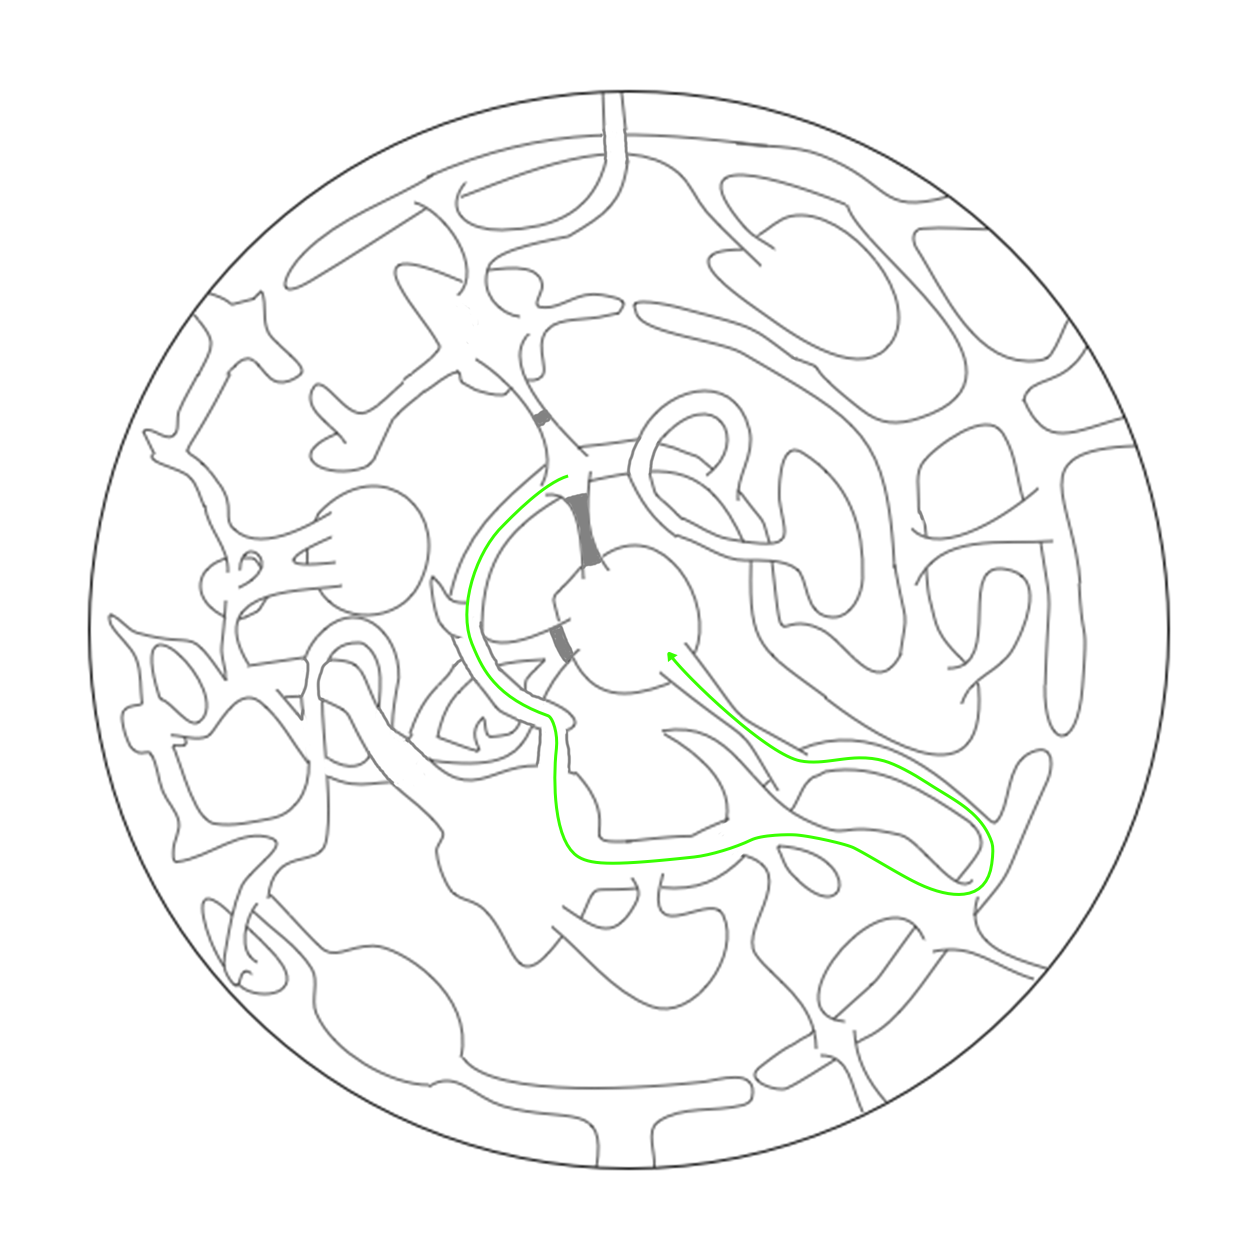
\includegraphics[width=0.7\linewidth]{images/map/map_principle_path_section_03.png}
	\caption*{Section 3 main path}
\end{figure}


\textbf{Encounter}
\begin{itemize}
	\item x1 NeoDemoGorgon
\end{itemize}
Just before entering the room, Elby will have chills down her spine. When Elby and \#010 will enter the den, after a brief iteration between the two, the NeoDemoGorgon will awaken and charge the player aggressively. Upon reaching the 50\% life threshold, the beast will start using the same dimensional travel power as the original one, only limited inside the den. Defeated the beast, Elby will go berserk and starts mutilating the corpse of the NeoDemoGorgon, until \#010 manages to calm her down.

\begin{itemize}
	\item 17 - 50\% Demorat, 30\% Demobat, 20\% Demodog
	\item 18 - Democerberus x1
	\item 19 - 15\% Demowolves, 35\% Demobat, 50\% Demodog
	\item 20 - 50\% Demorat, 30\% Demobat, 20\% Demodog
	\item 21 - 40\% Demorat, 40\% Demobat, 20\% Demomoles
	\item 22 - 50\% Demomoles, 25\% Demobat, 25\% Demodog
\end{itemize}

\textbf{Sounds}\\
The rustling of moving vines is more intense than Section 2, and a sound similar to the noise of a falling tree can be heard randomly. Elby makes a squelching sound when she walks on a organic branch.

\begin{itemize}
	\item 8 - Monster roar
	\item 9 - Rustling branches
\end{itemize}

\textbf{Lighting}\\
The environment is lit up with a bright red light emitted from the core. The same light shines slightly from the vines coming from the center of the pit, giving the impression of coming from a liquid similar to blood.

\begin{itemize}
	\item 3 - Trigger light change
\end{itemize}

\textbf{Drops}
\begin{itemize}
	\item 18 - Rotten potion
	\item 19 - Fresh potion
	\item 20 - Fresh elisir
	\item 21 - Fresh elisir
\end{itemize}
\newpage


\subsubsection{Giant Chasm Core}
The Core room is located in the center of the Giant Chasm, it has a circular shape with a diameter of 50m. In the center of the room stands the heart of the upsidedown, four times Elby high and at least three times wide, in front of which \#001 awaits the arrival of the player.

\vspace*{0.3cm}
\begin{figure}[H]
	\centering
	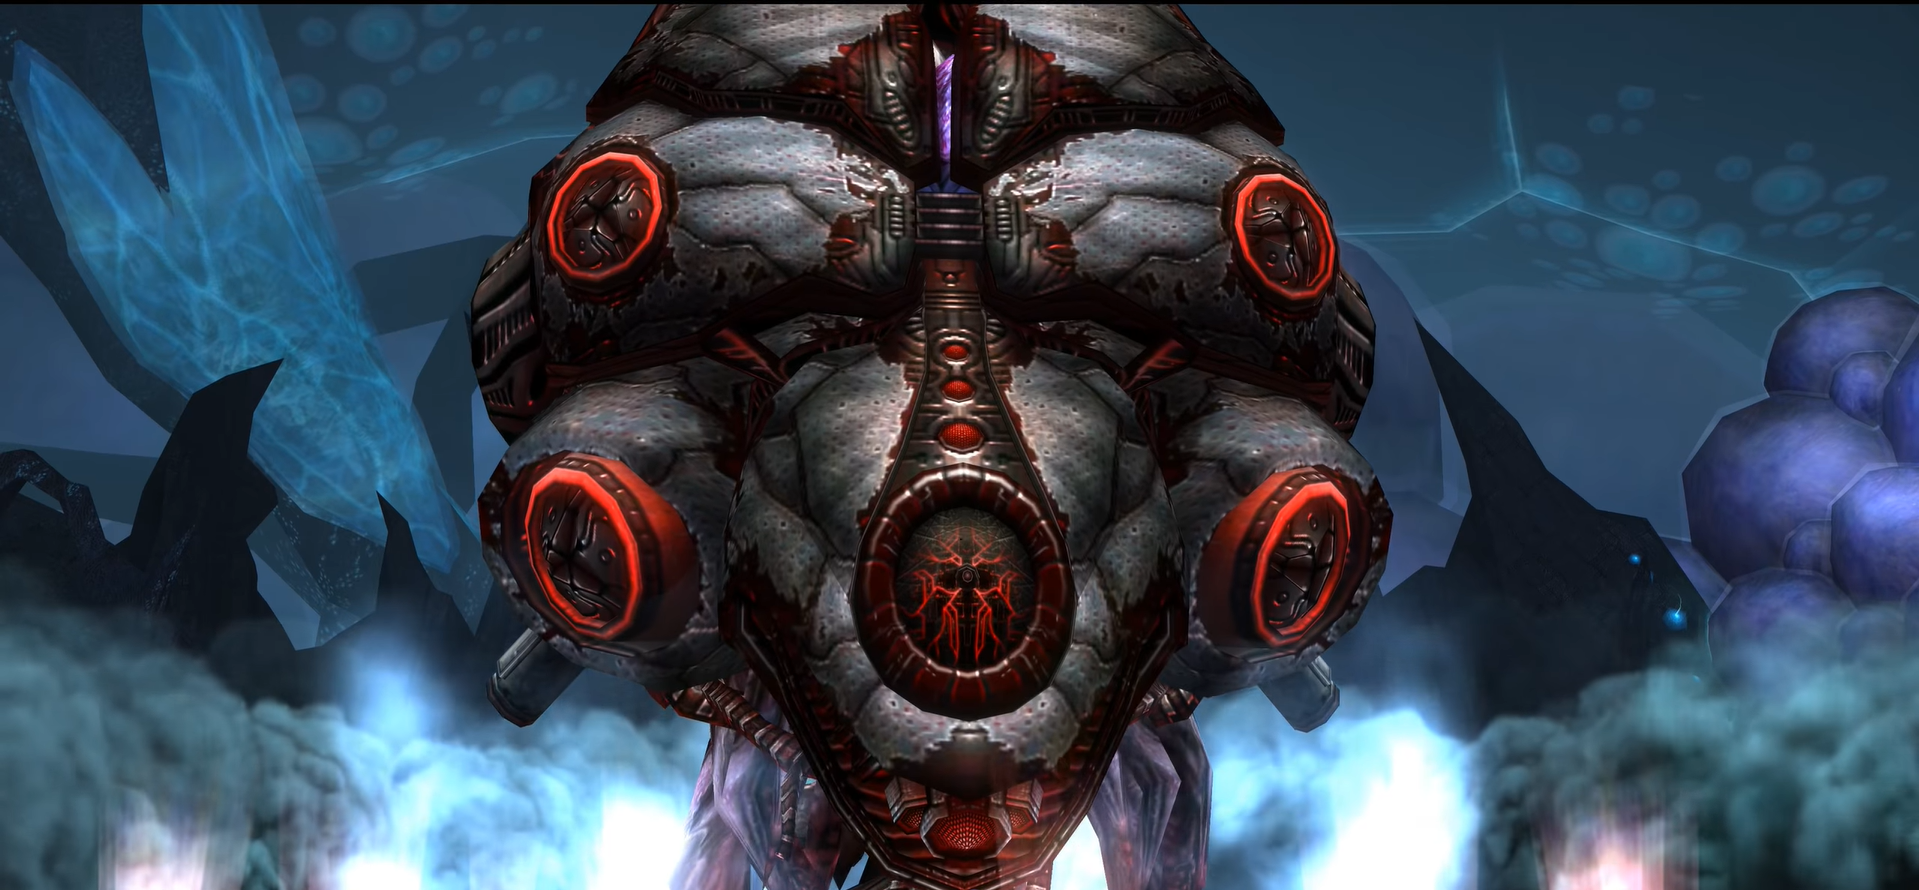
\includegraphics[width=0.8\linewidth]{images/visual_ref/15_giant_chasm/chasm_core.png}
	\caption*{Core of the Upside-Down (in-game it will be more organic and it will emit more red light)}
	\caption{ \textit{[Metroid Prime]}}
\end{figure}

\begin{figure}[H]
	\centering
	\includegraphics[width=0.8\linewidth]{images/visual_ref/15_giant_chasm/pallette/pallette_section_04.png}
\end{figure}

\begin{figure}[H]
	\centering
	\includegraphics[width=0.7\linewidth]{images/map/2D_map_section_04.png}
	\caption*{Boss room}
\end{figure}
\newpage


\subsection{Dialogues}

\subsubsection{Section 1}
\vspace*{0.3cm}

	\textbf{Entered the Giant Chasm, Elby and \#010 remain stunned by the dense network of ramifications that cover the whole area.}

\begin{dialogue}
	
	\speak{\#010} \direct{Astonished} \textit{"So this is the place where the core of the upside-down resides. It looks like a giant crater, it is possible that ..."}
	\speak{Elby} \textit{"I have no time or interest in your hypotheses, we must reach Kyle."}
	\speak{\#010} \textit{"Oh, you're right ... I see a light in the center, I think it's our destination"}\\
	
	\textbf{After a quick inspection, the two decide to continue along the edge and look for a route to the center.}\\
	
	If the player tries to go on the right:
	\speak{\#010} \textit{"This tangle of vines is too thick, we will not be able to pass this way. Let's find another path."}\\
	
	\textbf{Reached the remains of a building that collapsed inside the crater, Elby and 10 arrive in what appears to be
an old ballroom. Suddenly they hear the roars of monsters, which appear one after another around them.}\\
	
	
	\speak{\#010} \direct{Worried} \textit{"We are in their den after all, just try to save as much stamina as possible!"}\\
	
	\textbf{Once the monsters are defeated, they continue along the cliff to reach a second room divided in half
from a pit.}\\
	
	\speak{\#010} \textit{"I don't think I can jump so much, I'm sorry ..."}
	\speak{Elby} \textit{(That branch ... Maybe with my skills I can create a path)}\\
	
	\textbf{After using his telekinesis to cross the pit, Elby and \#010 follow the ramifications to continue on the track until they reach a third room, where they find several monsters impaled by vines.}\\
	
	
	\speak{\#010} \textit{"All these pierced monsters, I think it was \refer{\#001.}"}
	\speak{Elby} \textit{"You should be happy."}
	\speak{\#010} \textit{"Why?"}
	\speak{Elby} \textit{"..."}
	\speak{\#010} \textit{"Ah, if he killed them it means he doesn't have the power to control them, so \refer{\#005} is still alive!"}
	\speak{Elby} \direct{Nods towards \refer{\#010}}\\
	
	
	\textbf{Once at a dead end, they begin to look for a route inland.}\\
	
	
	\speak{\#010} \textit{"This is the only point from which we could descend, but the vines are too thick! Do you have any ideas?"}
	\speak{Elby} \direct{Looks around}
	\speak{Elby} \direct{Indicates a building on the edge of the crater}
	\speak{Elby} \direct{Smiling}\textit{"Freeze it"}
	\speak{\#010} \direct{Excited} \textit{"Maybe by combining our skills we can bring it down. Let's try!"}\\
	
	
	\textbf{After freezing the vines that stabilized the structure and having destroyed them by means of telekinesis, the building begins to collapse and the debris, after rolling along the wall, hit the barrier of vines, opening a gap.}\\
	
	
	\speak{\#010} \textit{"Now we can pass, but let's stay on guard."}
	
\end{dialogue}


\subsubsection{Section 2}
\vspace*{0.3cm}

\begin{dialogue}
	\speak{\#010} \direct{Coff coff}
	\speak{Elby} \textit{"The density of the air has changed, we are getting closer"}\\
	
	Entering the Safe Room:
	\speak{\#010} \direct{Relieved}\textit{"We should be safe in here, we can make a brief stop to regain strength"}\\
	
	Leaving the Safe Room:
	\speak{\#010} \textit{"Let's go, we should be halfway there"}
\end{dialogue}


\subsubsection{Section 3}
\vspace*{0.3cm}


	\textbf{The proximity to the core is increasingly evident: the ground is completely covered with organic vines and the air density is skyrocketing.}

\begin{dialogue}
	
	
	\speak{\#010} \textit{"We're getting closer to the core, the light that emanates is much more intense than before"}
	\speak{Elby} \direct{Angered} \textit{"Don't distract yourself!"}
	\speak{\#010} \textit{"Sorry!"}\\
	
	
	\textbf{Unable to follow the ground path, Elby and \#010 decide to continue the journey using the ramifications of the core as a route}\\
	
	\speak{\#010} \textit{"The branching of the core is extremely dense at this point"}
	\speak{Elby} \textit{"We are almost there"}\\
	
	Section one link, post skill:
	\speak{\#010} \textit{"We can now reach the entrance from here"}
	\speak{Elby} \direct{nods}\\
	
	
	\textbf{Finally they arrive on a non-natural path, certainly created by Kyle to reach the center of the giant chasm.}\\
	
	\speak{\#010} \textit{"\refer{\#001} must be close, are you ready?"}
	\speak{Elby} \textit{"Yes"} or \textit{"Not yet"}\\
	
	If answer is "Yes":
	\speak{\#010} \textit{"Ok, let's go ..."}\\
	
	If answer is "Not yet":
	\speak{\#010} \textit{"Make it quick, \refer{\#005} needs us!"}
	
\end{dialogue}


\subsubsection{Inner Section}
\vspace*{0.3cm}

\begin{dialogue}
	
	\speak{\#010} \textit{"\#001!"}
	\speak{Kyle} \direct{Joking} \textit{"Oh, finally. I was starting to think you were dead along the way!"}
	\speak{\#005} \direct{Squirms}
	\speak{Kyle} \textit{"Hey hey, calm down, wait for your turn"}\\
	
	If the player has visited Kyle's lab:
	\speak{\#010} \textit{"We've been in your lab, we know what you've done and what you are up to!"}
	\speak{Kyle} \textit{"So you found out everything ... Great, you saved me a lot of explanations"}\\
	
	If the player has not visited Kyle's lab:
	\speak{\#010} \textit{"Why all this?"}
	\speak{Kyle} \textit{"I just want back what was taken from me, nothing more"}\\
	
	\speak{\#010} \textit{"And are you going to kill us all for your purpose?"}
	\speak{Kyle} \textit{"Not everyone, just the two of them in case they don't want to cooperate" \direct{Points \refer{Elby} and \refer{\#005}}}
	\speak{Kyle} \textit{"By the way, you are staring at me with a fierce look, do you have something to say?" \direct{Watching \refer{Elby}}}
	\speak{Elby} \direct{Really angered} \textit{"Friends ... don't ... LIE !!!"} \direct{Gust of energy}
	\speak{Kyle} \textit{"Haha, so you consider me a friend, how nice!"}
	\speak{Kyle} \direct{Serious look}
	\speak{Kyle} \textit{"Chatting time's over, now give me your powers!"}
	
\end{dialogue}

\subsubsection{After Boss Fight}
\vspace*{0.3cm}

\begin{dialogue}
	\speak{Kyle} \textit{"... The effect of the core is more intense than I thought ..."}
	\speak{Elby} \textit{"Free \#005. NOW!"}
	\speak{Kyle} \textit{"..."}
	
	\textbf{The costrinctions around 005 are released, allowing him to move.}\\
	
	\speak{\#005}: \textit{"Thank y-"}\\
	
	\textbf{\#005 stops moving and suddenly blood starts to come out of his mouth.}\\
	
	\speak{Kyle} \textit{"You didn't give me a choice."}\\
	
	\textbf{A branch pierces the chest of \#005, extracting a DemoParasite.}\\
	
	\speak{\#010} \direct{Desperate look and vomit from horror}
	\speak{Elby} \direct{Tear from left eye}
	\speak{Kyle} \textit{"And now ..."}
	\speak{Kyle} \direct{swallows the DemoParasite}
	\speak{Kyle} \direct{closes his eyes}\\
	
	\textbf{Elby launches a mental attack, but a barrier of vines block it}\\
	\speak{Elby} "???!!?"
	\speak{Kyle} \direct{Open his eyes}
	\speak{Kyle} \textit{"I have control over the core, there's nothing more you can do."}\\
	
	\textbf{The whole Giant Chasm begins to tremble. In a few moments, hundreds of vines emerge from the ground, trapping Elby and \#010.}\\
	
	\speak{Kyle} \textit{"If you do not want to follow the same fate as \refer{\#005} do not resist and open the portal"}\\
	
	\textbf{A branch wraps around the neck of \#010, starting to strangle him}\\
	
	\speak{Elby} \direct{Initially reluctant} \textit{"Okay. I'll do it ..."}
	\speak{Kyle} \textit{"Great!"}\\
	
	\textbf{Kyle closes his eyes again, entering a state of deep concentration. Suddenly, the air inside the core changes, almost as if all the space there was in a continuos changing state}\\
	
	\speak{Kyle} \textit{"The time is right. Go on!"}\\
	
	\textbf{Elby starts to focus. The chasm begins to tremble again and in few seconds a portal appears in the room. Kyle watches it with a satisfied look and tears running down his face.}\\
	
	\speak{Kyle} \textit{"Now I can finally go home ..."}
\end{dialogue}

\section{Additional Mechanics}

\subsection{HUD}

\begin{figure}[H]
	\centering
	\includegraphics[width=14cm]{images/hud/HUD_life_green.png}
\end{figure}

Alongside Elby's health bar (the green one in the picture above), players will see in the HUD also the energy bar (the yellow one in the picture). “Energy” represent the amount of Elby’s telekynesis power, and it decreases when she uses her prowness to perform an active skill (see paragraph x).\\\\
A unique mechanic of this game is applied when Elby runs out of energy. The player is still allowed to make use of the active abilities drawing on the character's HP bar instead of using energy.\\
This double-edged sword allows the player to extend combat and exploration, but makes him vulnerable to fatal monster attacks.
Therefore energy is essential for survival and for this reason we have decided to add an auto-recovery that allows the latter to regenerate over time, specifically 1 NRG/turn.



\begin{figure}[H]
	\centering
	\includegraphics[width=14cm]{images/hud/HUD_life_orange.png}
	\caption*{HP > 25\% and HP $\leq$ 50\%}
\end{figure}

\begin{figure}[H]
	\centering
	\includegraphics[width=14cm]{images/hud/HUD_life_red.png}
	\caption*{HP $\leq$ 25\%}
\end{figure}

The picture of Elby inside the circle of the HUD changes accordingly to the status of the energy bar. Her facial expression changes when she is in combat and her energy has dropped under 20\%. In this case the figure will show blood dripping from the nose and will remain so until the fight is finished and the energy restored. For example, in the image above, Elby maintains the standard avatar although her life has fallen below 20\% (in this specific case the edge of the game screen will start to flash red).

\subsection{Skills and Items}
During the adventure, the player will unlock several Elby abilities, called Active Skills. These skills can be assigned as the player wishes in the 4 slots available in the Active Skills section of the HUD and can be changed everytime Elby visits a checkpoint. We made this choice because we wanted to allow the player to create a personalized set.\\\\
Sometimes elby will meet characters who decide to follow her on the journey. These NPCs have unique abilities, called Support Skills, which will be displayed in the Support Skills section of the HUD and they can not be changed. Every Support Skill will be explained below.\\\\
Items can be also be set in the Active Skills's HUD section, letting the player decide whether to use multiple skills with few objects or vice versa.\\\\
Being that a turn corresponds to 3 seconds, both Active and Support Skills provide a multiple cooldown of 3 based on the skill damage and effect.

\subsection{Items and crafting}

\subsubsection{Consumable items}

\subsubsection{Initial inventory prediction}
The potential inventory of the player at the beginning of the level could be:
\begin{itemize}
	\item Coal x2
	\item Fresh root x2
	\item Demorat tail x1
	\item Stick x3
	\item Bracelet x1
	\item Small potion x1
	\item Energy potion x1
	\item Bag x1
	\item Rock x3
	\item Demodog meat x2
	\item Sand x1
\end{itemize}

\subsubsection{Collectible items}

\newpage

\subsection{Checkpoints and Game Saves}

\begin{figure}[H]
	\centering
	\includegraphics[width=14cm]{images/visual_ref/checkpoint.png}
\end{figure}

Scattered around the levels players can find safe places to take refuge and light a bonfire. These spots act as checkpoints.\\
In the Giant Chasm there are 3 of them, located in the Cerberus room (activated only after defeating the miniboss), at the beginning of the second section of the level and in the middle of the third section.\\
While Elby is at the bonfire, she can cook food, craft items, change her active skills and rest, fully recovering both hit points and mana points, allowing however the respawn of all the monsters in the section (only if they have been previously defeated).\\
We have decided not to allow the player to use quick travel between the various checkpoints on the map to remain consistent with the theme of the game (the player can still use it to move between the game areas). We also thought that the best solution for saving the game is an auto-save every time the player visits a bonfire. This allows us to predict the player's actions and movements with more precision, incentivize him to plan a strategy to cross the maps and prevent him from passing certain key points of the level simply by saving and repeating, consequently increasing the difficulty and the overall challenge.





\end{document}
